% ============================================================================
% causalGBKMR -- Software Paper for Environmental Health Perspectives (EHP)
%
% First-author dissertation paper introducing the CausalBKMR R commands
% for time-varying environmental mixtures within the causalmixtures package.
%
% EHP Research Article requirements:
%   - Main text: <= 7,000 words (excluding abstract/refs/tables/captions/supp)
%   - Structured abstract: <= 300 words
%   - No official LaTeX template; use clean article class for Overleaf
% ============================================================================
\documentclass[11pt]{article}

% --- Packages ---------------------------------------------------------------
\usepackage[utf8]{inputenc}
\usepackage[T1]{fontenc}
\usepackage{lmodern}
\usepackage[a4paper,margin=1in]{geometry}
\usepackage{amsmath,amssymb,amsthm}
\usepackage{graphicx}
\usepackage{booktabs}
\usepackage{caption}
\usepackage{subcaption}
\usepackage{hyperref}
\usepackage{authblk}
\usepackage{lineno}
\usepackage{xcolor}
\usepackage{listings}
\usepackage{setspace}
\usepackage{xurl}
\usepackage{tikz}
\usepackage{verbatim}
\usetikzlibrary{arrows.meta,positioning,bending}

\hypersetup{
  colorlinks=true,
  linkcolor=blue!60!black,
  citecolor=blue!60!black,
  urlcolor=blue!60!black
}

% Numeric reference style for EHP-like citations
\usepackage[numbers,super,sort&compress]{natbib}
\bibliographystyle{unsrtnat}

% R code listing
\lstdefinestyle{Rstyle}{
  language=R,
  basicstyle=\ttfamily\small,
  keywordstyle=\color{blue},
  commentstyle=\color{gray},
  stringstyle=\color{red!60!black},
  showstringspaces=false,
  breaklines=true,
  frame=single,
  rulecolor=\color{gray!30}
}
\lstset{style=Rstyle}

\newcommand{\todo}[1]{{\color{red}\textbf{[TODO: #1]}}}
\newcommand{\note}[1]{{\color{purple}\textit{[#1]}}}
\newcommand{\pkg}[1]{\texttt{#1}}
\newcommand{\code}[1]{\texttt{#1}}
\newcommand{\fn}[1]{\texttt{#1()}}

\linenumbers
\onehalfspacing
\emergencystretch=3em

% --- Title and authors ------------------------------------------------------
\title{CausalBKMR: R Commands for Causal Inference\\ with Time-Varying Environmental Mixtures}

\author[1]{Yanran Li}
\author[1]{Arce Domingo-Relloso}
\author[1,2]{Zilan Chai}
\author[3]{Ana Navas-Acien}
\author[4]{Brent A.\ Coull}
\author[1,5,*]{Linda Valeri}

\affil[1]{Department of Biostatistics, Columbia University Mailman School of Public Health, New York, NY, USA}
\affil[2]{Microsoft, Redmond, WA, USA}
\affil[3]{Department of Environmental Health Sciences, Columbia University Mailman School of Public Health, New York, NY, USA}
\affil[4]{Department of Biostatistics, Harvard T.H.\ Chan School of Public Health, Boston, MA, USA}
\affil[5]{Department of Epidemiology, Harvard T.H.\ Chan School of Public Health, Boston, MA, USA}
\affil[*]{Corresponding author: \href{mailto:lv2424@columbia.edu}{lv2424@columbia.edu}}

\date{\today}

\begin{document}
\maketitle

% ============================================================================
% STRUCTURED ABSTRACT
% EHP guidelines call for Background / Objectives / Methods / Results / Discussion.
% Current draft uses Background / Methods / Results / Conclusions (Bobb-2018 style).
% TODO: decide whether to restructure into the EHP 5-heading format before submission.
% ============================================================================
\begin{abstract}
\noindent\textbf{Background.} Environmental health studies increasingly collect repeated measurements of correlated chemical exposures, biomarkers, and health outcomes. These data raise two linked challenges: exposures occur as mixtures that may act nonlinearly and interactively, and time-varying confounders may be affected by earlier exposure while confounding later exposure--outcome associations. Existing R software addresses either environmental mixtures or longitudinal causal inference, but not an automated g-formula implementation of Bayesian kernel machine regression for time-varying mixtures.

\noindent\textbf{Methods.} \pkg{CausalBKMR} implements g-BKMR, which combines the parametric g-formula with Bayesian kernel machine regression to estimate average causal effects comparing full exposure-mixture trajectories. \pkg{CausalBKMR} is being developed as the time-varying mixture module of the broader \pkg{causalmixtures} package, complementing existing commands for BKMR-based causal mediation analysis and multiple-imputation BKMR. The module accepts longitudinal mixture exposures, time-varying confounders, baseline covariates, and continuous or binary outcomes, fits sequential BKMR models for the confounder and outcome processes, and simulates counterfactual outcome distributions under user-specified exposure trajectories. For large continuous-outcome analyses, the module can call a fastBKMR engine through \pkg{fbkmr}.

\noindent\textbf{Results.} A six-scenario simulation study with continuous and binary outcomes shows that \pkg{CausalBKMR} consistently exhibits low bias and near-nominal coverage across linear, quadratic, and interaction-driven exposure-response surfaces, performing comparably to the parametric g-formula with correct model specification and outperforming traditional regression, the misspecified parametric g-formula, and BKMR with time-grouped variable selection. In an application to the Strong Heart Study, we estimate the joint causal effect of six urinary metals measured at three visits on log fasting blood glucose: the 75th-versus-25th percentile contrast was $1.01$ standardised units (95\% credible interval: $0.72$, $1.33$), with zinc identified as the dominant contributor across all visits. A separate computational benchmark on MESA-scale data ($n = 6{,}000$) shows that the optional fastBKMR engine completes a full three-model g-formula sequence in approximately 50 minutes on 10 cores while recovering posterior summaries consistent with the standard \pkg{bkmr} engine and yielding 5--10 times lower between-replication variance than a single $n = 500$ subsample fit.

\noindent\textbf{Conclusions.} \pkg{CausalBKMR} will extend \pkg{causalmixtures} to time-varying environmental mixtures under longitudinal confounding. The module fills a gap between mixture-analysis packages and longitudinal g-formula packages by providing a single command family for data preparation, model fitting, counterfactual simulation, diagnostics, and interpretation.

\vspace{0.5em}
\noindent\textbf{Keywords:} Bayesian kernel machine regression; causal inference; environmental mixtures; g-formula; longitudinal data; R software.
\end{abstract}

% ============================================================================
% BACKGROUND
% ============================================================================
\section*{Background}
\label{sec:background}

Environmental epidemiology studies often measure multiple correlated exposures repeatedly over time. In studies of metals, air pollution, endocrine-disrupting chemicals, or dietary contaminants, the scientific question is rarely whether one exposure at one time point is associated with the outcome. Investigators instead ask how a mixture history affects a later health outcome, whether the effect is nonlinear, and whether the same chemical contributes differently across developmental windows or clinical visits.

Longitudinal mixtures create a causal problem that is not solved by adding all repeated exposures and covariates to a conventional regression model. Time-varying covariates can be affected by earlier exposure and can also predict later exposure and the outcome. Conditioning naively on these covariates may block part of the exposure effect or introduce bias, whereas failing to account for them may leave time-varying confounding uncontrolled. Figure~\ref{fig:dag} summarizes the target data structure: baseline covariates $C_0$ influence the exposure mixture $A_t$, time-varying confounders $L_t$, and outcome $Y$; earlier mixtures affect later confounders; and later confounders affect subsequent mixtures and the final outcome.

Several R packages support related pieces of this problem. The \pkg{bkmr} package implements Bayesian kernel machine regression for flexible analysis of correlated exposure mixtures, including nonlinear exposure-response surfaces, interactions, and posterior inclusion probabilities \citep{bobb_bkmr_2018}. The \pkg{qgcomp} and \pkg{gWQS} packages implement index-based mixture methods that estimate interpretable joint mixture effects under more structured regression assumptions \citep{qgcomp_package,gwqs_package}. The \pkg{causalmixtures} package provides a suite of BKMR-based commands for causal mixture analyses, currently organized around BKMR-CMA for causal mediation analysis and BKMR-MI for analyses with multiple imputation \citep{causalmixtures_package}. For longitudinal causal inference, \pkg{gfoRmula} and related g-formula software estimate effects of time-varying treatment strategies under measured time-varying confounding \citep{mcgrath_gformula_2020,gformula_package}, but these tools do not provide a BKMR mixture-response model as the core exposure-response engine. Thus, existing software covers flexible mixture modeling, BKMR-based mediation and missing-data workflows, or longitudinal g-formula estimation, but does not provide an automated implementation of g-BKMR for time-varying environmental mixtures.

\pkg{CausalBKMR} fills this software gap as the planned third module of \pkg{causalmixtures}. The module implements the g-BKMR estimator proposed by \citet{chai_gbkmr} and provides R commands for data preparation, input auditing, sequential BKMR fitting, Monte Carlo g-computation, posterior summaries, and diagnostic output. During development, these commands are documented on a separate \pkg{CausalBKMR} pkgdown site; in the integrated release, the documentation is intended to appear as a top-level \pkg{CausalBKMR} tab within the \pkg{causalmixtures} website.

% ============================================================================
% METHODS
% ============================================================================
\section*{Methods}
\label{sec:methods}

\subsection*{CausalBKMR estimator}
Consider $n$ individuals followed over $T$ visits. At visit $t$, let $A_t = (A_{t1}, \ldots, A_{tp})$ denote the $p$-component exposure mixture and let $L_t$ denote time-varying covariates that may be affected by earlier exposures and may confound future exposure--outcome relationships. Let $C_0$ denote baseline covariates and let $Y$ denote a final continuous or binary outcome. For two full exposure-mixture trajectories $\bar{\mathbf{a}} = (\mathbf{a}_0,\ldots,\mathbf{a}_{T-1})$ and $\bar{\mathbf{a}}^* = (\mathbf{a}^*_0,\ldots,\mathbf{a}^*_{T-1})$, the target estimand is the average causal effect
\[
  ACE = E\{Y(\bar{\mathbf{a}}^*)\} - E\{Y(\bar{\mathbf{a}})\}.
\]
The default contrast in the \pkg{CausalBKMR} command family compares all mixture components at the 75th percentile with all mixture components at the 25th percentile across all visits, although users can define component-specific and time-specific trajectories.

The estimator uses the longitudinal g-formula to express counterfactual outcome means through the observed-data distribution of the outcome and time-varying confounders. \pkg{CausalBKMR} fits this distribution sequentially. For each post-baseline time-varying confounder, the module fits a BKMR mediator model conditional on the exposure and covariate history. It then fits a BKMR outcome model conditional on the exposure and covariate history. Posterior draws from these models are used to simulate counterfactual confounder histories and outcomes under $\bar{\mathbf{a}}$ and $\bar{\mathbf{a}}^*$, producing posterior samples of $ACE$.

BKMR is used because the mixture-response function can be nonlinear and non-additive. In each BKMR model, the kernel component captures the joint effect of the mixture and relevant covariate history, while baseline covariates enter as linear terms. Variable selection can be incorporated through BKMR posterior inclusion probabilities, allowing the fitted outcome model to identify mixture components and time windows that contribute most strongly to the estimated response surface.

\subsection*{fastBKMR engine}
Standard BKMR can become computationally expensive when the sample size is large or when the longitudinal structure requires many sequential mediator models. For large continuous-outcome analyses, \pkg{CausalBKMR} can use \pkg{fbkmr} through the \code{engine = "fastbkmr"} option. The fastBKMR path implements the median-posterior subset-aggregation strategy of \citet{sonabend_fastbkmr_2026}, which fits Gaussian-kernel BKMR independently on multiple data subsets and combines posterior summaries through the median of subset posteriors.

\subsection*{Engine support and outcome--confounder types}
The two engines do not have identical support for outcome and time-varying-confounder types. Table~\ref{tab:engine_support} summarises the current policy. The standard \pkg{bkmr} engine accepts both continuous and binary outcomes, using a probit BKMR outcome model for the binary case. The \pkg{fbkmr} engine accepts only continuous outcomes; \code{gbkmr\_run()} raises a hard error if \code{engine = "fastbkmr"} is requested with a binary outcome, because the median-posterior aggregation strategy has been validated for the Gaussian case only. For binary time-varying confounders $L_t$, both engines fit the corresponding $L_t$ models as Gaussian and emit a warning, since the kernel infrastructure used for confounder models in the current release is Gaussian. Users with binary $L_t$ should treat the warning as a real modelling assumption and consider sensitivity analyses to discretisation thresholds.

\begin{table}[h]
\centering
\caption{Engine support for \code{gbkmr\_run()} as a function of outcome type and time-varying confounder type. The standard \pkg{bkmr} engine accepts both outcome types; the \pkg{fbkmr} engine accepts continuous outcomes only and raises a hard error otherwise. Binary time-varying confounders are fit as Gaussian by both engines with a warning.}
\label{tab:engine_support}
\begin{tabular}{llll}
\toprule
Outcome $Y$ & Confounder $L_t$ & \code{engine = "bkmr"} & \code{engine = "fastbkmr"} \\
\midrule
continuous & all continuous & Supported               & Supported \\
binary     & all continuous & Supported (probit $Y$)  & Hard error \\
continuous & any binary     & Warning ($L$ Gaussian)  & Warning ($L$ Gaussian) \\
binary     & any binary     & Warning (probit $Y$, $L$ Gaussian) & Hard error \\
\bottomrule
\end{tabular}
\end{table}

% ============================================================================
% SOFTWARE IMPLEMENTATION
% ============================================================================
\section*{Software implementation}
\label{sec:software}

\subsection*{R-command workflow}
\pkg{CausalBKMR} is designed as a small command family within \pkg{causalmixtures}. The recommended workflow is to convert user-supplied matrices into the module's wide longitudinal format with \code{prepare\_gbkmr\_data()}, inspect the detected structure with \code{detect\_variable\_patterns()}, and run the analysis with \code{gbkmr\_run()}. The lower-level function \code{run\_gbkmr\_panel()} is exported for advanced users who already understand the internal data layout, but it is not the recommended entry point for applied analyses.

\begin{verbatim}
library(causalmixtures)

prepared <- prepare_gbkmr_data(
  Y = Y,
  Z = Z,
  X = X,
  time_points = 3,
  mixture_components = 6,
  td_covariates = 2,
  baseline_covariates = 4,
  td_covariate_names = c("waist", "glucose")
)

detect_variable_patterns(prepared, T = 3)

fit <- gbkmr_run(
  data = prepared,
  outcome = "Y",
  outcome_type = "continuous",
  time_points = 3,
  engine = "auto",
  a_probs = c(0.25, 0.75),
  iter = 15000,
  K = 1000
)
\end{verbatim}

The input objects are deliberately simple. \code{Y} is an outcome vector, \code{Z} is an $n \times (pT)$ matrix of mixture exposures ordered by time, and \code{X} is an $n \times (L T + B)$ matrix containing time-varying covariates followed by baseline covariates. The preparation command standardizes the column naming convention, optionally log-transforms mixture variables, and stores metadata describing the number of visits, mixture components, time-varying covariates, and baseline covariates. Until the merge into \pkg{causalmixtures} is complete, the same command family is maintained on the development \pkg{CausalBKMR} documentation site.

\subsection*{Model fitting and output}
\code{gbkmr\_run()} audits the prepared data, chooses a fitting engine, fits the sequential mediator and outcome models, performs Monte Carlo g-computation, and returns an object of class \code{gbkmr\_results}. The output includes the posterior mean and credible interval for the causal contrast, counterfactual means under $\bar{\mathbf{a}}$ and $\bar{\mathbf{a}}^*$, variable-importance summaries, detected data structure, convergence diagnostics, raw model objects, and the original analysis settings.

For binary outcomes, users specify \code{outcome\_type = "binary"}. The standard BKMR engine then fits a probit BKMR outcome model and reports the causal effect on the probability scale as a risk difference. If a user requests \code{engine = "fastbkmr"} for a binary outcome, the command stops with an explicit error because the current fastBKMR path is Gaussian-only.

% ============================================================================
% PRACTICAL CONSIDERATIONS
% ============================================================================
\section*{Practical considerations}
\label{sec:practical}

\subsection*{Diagnostics}
Because \pkg{CausalBKMR} fits several Bayesian models within one longitudinal workflow, diagnostics should be treated as part of the analysis rather than as an optional post-processing step. The command prints an input audit before model fitting, including the detected outcome type, number of exposure components, number of time points, detected time-varying covariates, baseline covariates, selected engine, MCMC settings, and intervention contrast. This audit is intended to catch misspecified column ordering or unintended contrast definitions before a long MCMC run begins.

After fitting, the package prints the estimated causal effect, counterfactual means, model sequence, causal assumptions, and convergence checks. The current diagnostic layer reports effective sample size and Geweke statistics for fitted BKMR models. When diagnostics indicate poor mixing or nonstationarity, users should increase the number of MCMC iterations, use a later post-burn-in selection window, inspect trace plots, and consider simplifying highly unstable exposure or covariate histories.

\subsection*{Identifiability assumptions}
The numerical output of \pkg{CausalBKMR} has a causal interpretation only under standard longitudinal causal assumptions. Consistency requires the observed outcome under the observed exposure history to equal the corresponding counterfactual outcome. Sequential exchangeability requires no unmeasured time-varying confounding after conditioning on the measured exposure and covariate history at each visit. Positivity requires that the exposure trajectories being compared are supported within the observed covariate histories. These assumptions are not guaranteed by the command; they must be justified by study design, measurement quality, subject-matter knowledge, and sensitivity analyses.

\subsection*{Choosing exposure contrasts}
The contrast $\bar{\mathbf{a}}$ versus $\bar{\mathbf{a}}^*$ should represent a scientifically meaningful intervention on the mixture history. The default 25th-versus-75th percentile contrast is useful as a standardized summary of the joint mixture effect, but it may not be appropriate for all applications. When components have different toxicological interpretations, users may specify named vectors through \code{a\_vals} and \code{astar\_vals} to define component-specific and time-specific interventions. Contrasts should remain within the empirical support of the observed exposure distribution unless extrapolation is scientifically justified and clearly disclosed.

% ============================================================================
% RESULTS  (Simulation study + Strong Heart Study application)
% Simulation content mirrors causalGBKMR_EHP_app/sections/simulation.tex
% Application content mirrors causalGBKMR_EHP_app/sections/results_application.tex
% ============================================================================
\section*{Results}
\label{sec:results}

\subsection*{Simulation study}

We evaluate the ability of \pkg{CausalBKMR} to estimate the joint effect of a mixture in comparison to (i) the traditional regression approach with direct confounding adjustment in the outcome model, (ii) the parametric g-formula, (iii) the parametric g-formula with correct model specification, and (iv) BKMR with hierarchical variable selection grouped by time point (which ignores time-dependent confounding).

\subsubsection*{Setup}

A population dataset of $1{,}000{,}000$ observations was generated, where $\mathbf{A}_t = (A_{t,1}, \ldots, A_{t,k})^\top$ denotes the $k$-th metal exposure observed at the $t$-th time point. Baseline covariates $C_0$ and time-varying confounders $L_t$ were generated alongside. In each simulation, smaller datasets were randomly sampled from the population. Time-varying confounders were drawn from a normal distribution and log-transformed metal exposures from a multivariate normal distribution. Scenarios 1--4 considered two time points; scenarios 5--6 considered three time points (i.e., $t = 0, 1, 2$):
\begin{align*}
    \log A_0 &\sim N\!\left(h_{A_0}(C_0),\, \sigma^2_{A_0}\right), \\
    L_1 &\sim N\!\left(h_{L_1}(A_0, C_0),\, \sigma^2_{L_1}\right), \\
    \log A_1 &\sim N\!\left(h_{A_1}(A_0, L_1),\, \sigma^2_{A_1}\right), \\
    L_2 &\sim N\!\left(h_{L_2}(A_1, L_1),\, \sigma^2_{L_2}\right), \\
    \log A_2 &\sim N\!\left(h_{A_2}(A_1, L_2),\, \sigma^2_{A_2}\right).
\end{align*}

Two outcome types were considered, continuous and binary. The continuous outcome was generated by
\begin{equation*}
    y_i \sim N\!\left(h_Y(L_1, L_2, A_0, A_1, A_2),\, \sigma^2_Y\right),
\end{equation*}
and the binary outcome by
\begin{equation*}
    y_i \sim \text{Bin}\!\left(n,\, h_Y(L_1, L_2, A_0, A_1, A_2)\right).
\end{equation*}
Variances $\sigma^2_{A_t}$, $\sigma^2_{L_t}$, and $\sigma^2_Y$ were calibrated to be realistic based on the Strong Heart Study application. For the underlying exposure--confounder functions $h_{L_t}(\cdot)$ and exposure-response functions $h_{Y_t}(\cdot)$, we considered six scenarios for the continuous outcome and three additional scenarios for the binary outcome, varying linearity, strength of confounding, and presence of interactions. The specification of each scenario is summarised in Table~\ref{tab:sim_scenarios}.

\begin{table}[h]
\centering
\caption{Number of time points, the strength of the confounding effect, and exposure-confounder-response underlying relationships used for each simulation scenario.}
\label{tab:sim_scenarios}
\begin{tabular}{lccccc}
\toprule
Scenario & Time points & Correlation & Confounding & Underlying relationship & Outcome \\
\midrule
1 & 2 & moderate & low    & quadratic + interaction & continuous \\
2 & 2 & moderate & strong & linear                  & continuous \\
3 & 2 & moderate & strong & quadratic               & continuous \\
4 & 2 & moderate & low    & quadratic + interaction & binary     \\
5 & 3 & moderate & strong & quadratic               & binary     \\
6 & 3 & moderate & strong & linear                  & binary     \\
\bottomrule
\end{tabular}
\end{table}

For each scenario, $500$ datasets of $500$ observations were sampled from the population dataset. We first fit the BKMR confounder and outcome models:
\begin{align}
    L_{1i} &= h_L(\mathbf{A}_{0i}) + \mathbf{C}_i^\top \boldsymbol{\beta} + \epsilon_{L_{1i}}, \label{eq:sim_L1} \\
    L_{2i} &= h_L(\mathbf{A}_{0i}, \mathbf{A}_{1i}, \mathbf{L}_{1i}) + \mathbf{C}_i^\top \boldsymbol{\beta} + \epsilon_{L_{2i}}, \label{eq:sim_L2} \\
    Y_i &= h_Y(\mathbf{A}_{0i}, \mathbf{A}_{1i}, \mathbf{A}_{2i}, \mathbf{L}_{1i}, \mathbf{L}_{2i}) + \mathbf{C}_i^\top \boldsymbol{\theta} + \epsilon_{Y_i}. \label{eq:sim_Y}
\end{align}
Using \pkg{CausalBKMR}, we estimated the change in the potential outcome $Y$ for a shift of the exposure mixture from $\mathbf{a}$ (all exposures at the $25^{\text{th}}$ percentile of the underlying dataset) to $\mathbf{a}^*$ (all exposures at the $75^{\text{th}}$ percentile of the underlying dataset).

We compare the performance of the following six methods: (1) CausalBKMR with variable selection; (2) CausalBKMR without variable selection; (3) parametric g-formula with correct model specification; (4) traditional regression---linear or logistic regression with direct adjustment for all exposures and confounders at all time points; (5) parametric g-formula adjusting for all exposures and covariates; and (6) BKMR with hierarchical variable selection grouped by time points.

\subsubsection*{Simulation results}

Tables~\ref{tab:sim_continuous} and~\ref{tab:sim_binary} summarise the empirical bias, mean squared error (MSE), and coverage probabilities of the average treatment effect estimates across the $500$ simulated datasets. Figure~\ref{fig:sim_results} visualises these results.

The parametric g-formula with correct model specification yielded low bias and high coverage, as expected. However, in real-world applications the true functional form is unknown, particularly when relationships involve quadratic terms or interactions; thus, although the correctly specified g-formula is a useful benchmark in simulation, its practical utility is limited. Traditional linear and logistic regression models exhibited substantial bias, particularly under nonlinear underlying relationships, because they cannot capture the time-varying structure of the data.

When the underlying relationship was linear (scenarios 2 and 6), coverage of the parametric g-formula was reasonable; otherwise (scenarios 1, 3, 4, 5), coverage dropped sharply, reflecting the heavy reliance of the parametric g-formula on correct model specification. \pkg{CausalBKMR} consistently exhibited low bias across scenarios, comparable to the correctly specified g-formula benchmark. \pkg{CausalBKMR} with and without variable selection produced similar bias and coverage in most cases; the no-selection variant slightly outperformed in some scenarios but at substantially higher computational cost (it estimates effects for all predictors rather than a selected subset). We therefore recommend \pkg{CausalBKMR} with variable selection in practice. BKMR with grouped variable selection exhibited the highest bias and lowest coverage among all methods, particularly under strong confounding, because it ignores time-varying confounding.

\begin{table}[h]
\centering
\caption{Bias, mean squared error (MSE), and coverage probabilities of the ATE estimates from our simulation under varying underlying relationships with a continuous outcome. Comparison of \pkg{CausalBKMR} with and without variable selection, the parametric g-formula, traditional linear regression, BKMR with grouped variable selection, and the parametric g-formula with correct model specification.}
\label{tab:sim_continuous}
\begin{tabular}{cl rrr}
\toprule
Scenario & Method & Bias & MSE & Coverage \\
\midrule
1 & CausalBKMR              &  0.00 & 0.01 & 0.98 \\
1 & g-formula               &  0.26 & 0.08 & 0.44 \\
1 & Linear model            &  0.26 & 0.08 & 0.47 \\
1 & BKMR-group              & $-0.02$ & 0.01 & 0.91 \\
1 & CausalBKMR (no varsel)  & $-0.00$ & 0.02 & 0.99 \\
1 & g-formula (correct)     &  0.01 & 0.01 & 0.93 \\
\midrule
2 & CausalBKMR              &  0.01 & 0.03 & 0.96 \\
2 & g-formula               & $-0.14$ & 0.04 & 0.84 \\
2 & Linear model            & $-0.14$ & 0.04 & 0.81 \\
2 & BKMR-group              & $-0.02$ & 0.63 & 0.01 \\
2 & CausalBKMR (no varsel)  & $-0.02$ & 0.04 & 0.99 \\
2 & g-formula (correct)     & $-0.00$ & 0.02 & 0.95 \\
\midrule
3 & CausalBKMR              & $-0.13$ & 0.05 & 0.91 \\
3 & g-formula               &  0.76 & 0.64 & 0.11 \\
3 & Linear model            & $-0.38$ & 0.25 & 0.78 \\
3 & BKMR-group              &  1.19 & 1.47 & 0.00 \\
3 & CausalBKMR (no varsel)  & $-0.11$ & 0.07 & 0.99 \\
3 & g-formula (correct)     &  0.09 & 0.03 & 0.95 \\
\bottomrule
\end{tabular}
\end{table}

\begin{table}[h]
\centering
\caption{Bias, mean squared error (MSE), and coverage probabilities of the ATE estimates from our simulation under varying underlying relationships with a binary outcome. Comparison of \pkg{CausalBKMR} with and without variable selection, the parametric g-formula, traditional logistic regression, BKMR with grouped selection, and the parametric g-formula with correct model specification.}
\label{tab:sim_binary}
\begin{tabular}{cl rrr}
\toprule
Scenario & Method & Bias & MSE & Coverage \\
\midrule
4 & CausalBKMR              &  0.03 & 0.00 & 0.77 \\
4 & g-formula               &  0.03 & 0.00 & 0.80 \\
4 & Linear model            & $-0.25$ & 0.09 & 0.68 \\
4 & BKMR-group              &  0.03 & 0.00 & 0.81 \\
4 & CausalBKMR (no varsel)  &  0.01 & 0.00 & 0.99 \\
4 & g-formula (correct)     & $-0.03$ & 0.00 & 0.83 \\
\midrule
5 & CausalBKMR              & $-0.02$ & 0.00 & 0.93 \\
5 & g-formula               &  0.08 & 0.14 & 0.78 \\
5 & Linear model            &  0.07 & 0.01 & 0.93 \\
5 & BKMR-group              &  0.08 & 0.01 & 0.45 \\
5 & CausalBKMR (no varsel)  &  0.01 & 0.00 & 0.97 \\
5 & g-formula (correct)     & $-0.02$ & 0.00 & 0.92 \\
\midrule
6 & CausalBKMR              & $-0.02$ & 0.00 & 0.94 \\
6 & g-formula               & $-0.10$ & 0.02 & 0.92 \\
6 & Linear model            &  0.04 & 0.01 & 0.95 \\
6 & BKMR-group              &  0.07 & 0.01 & 0.79 \\
6 & CausalBKMR (no varsel)  &  0.00 & 0.00 & 0.98 \\
6 & g-formula (correct)     & $-0.02$ & 0.00 & 0.93 \\
\bottomrule
\end{tabular}
\end{table}

\begin{figure}[h]
\centering
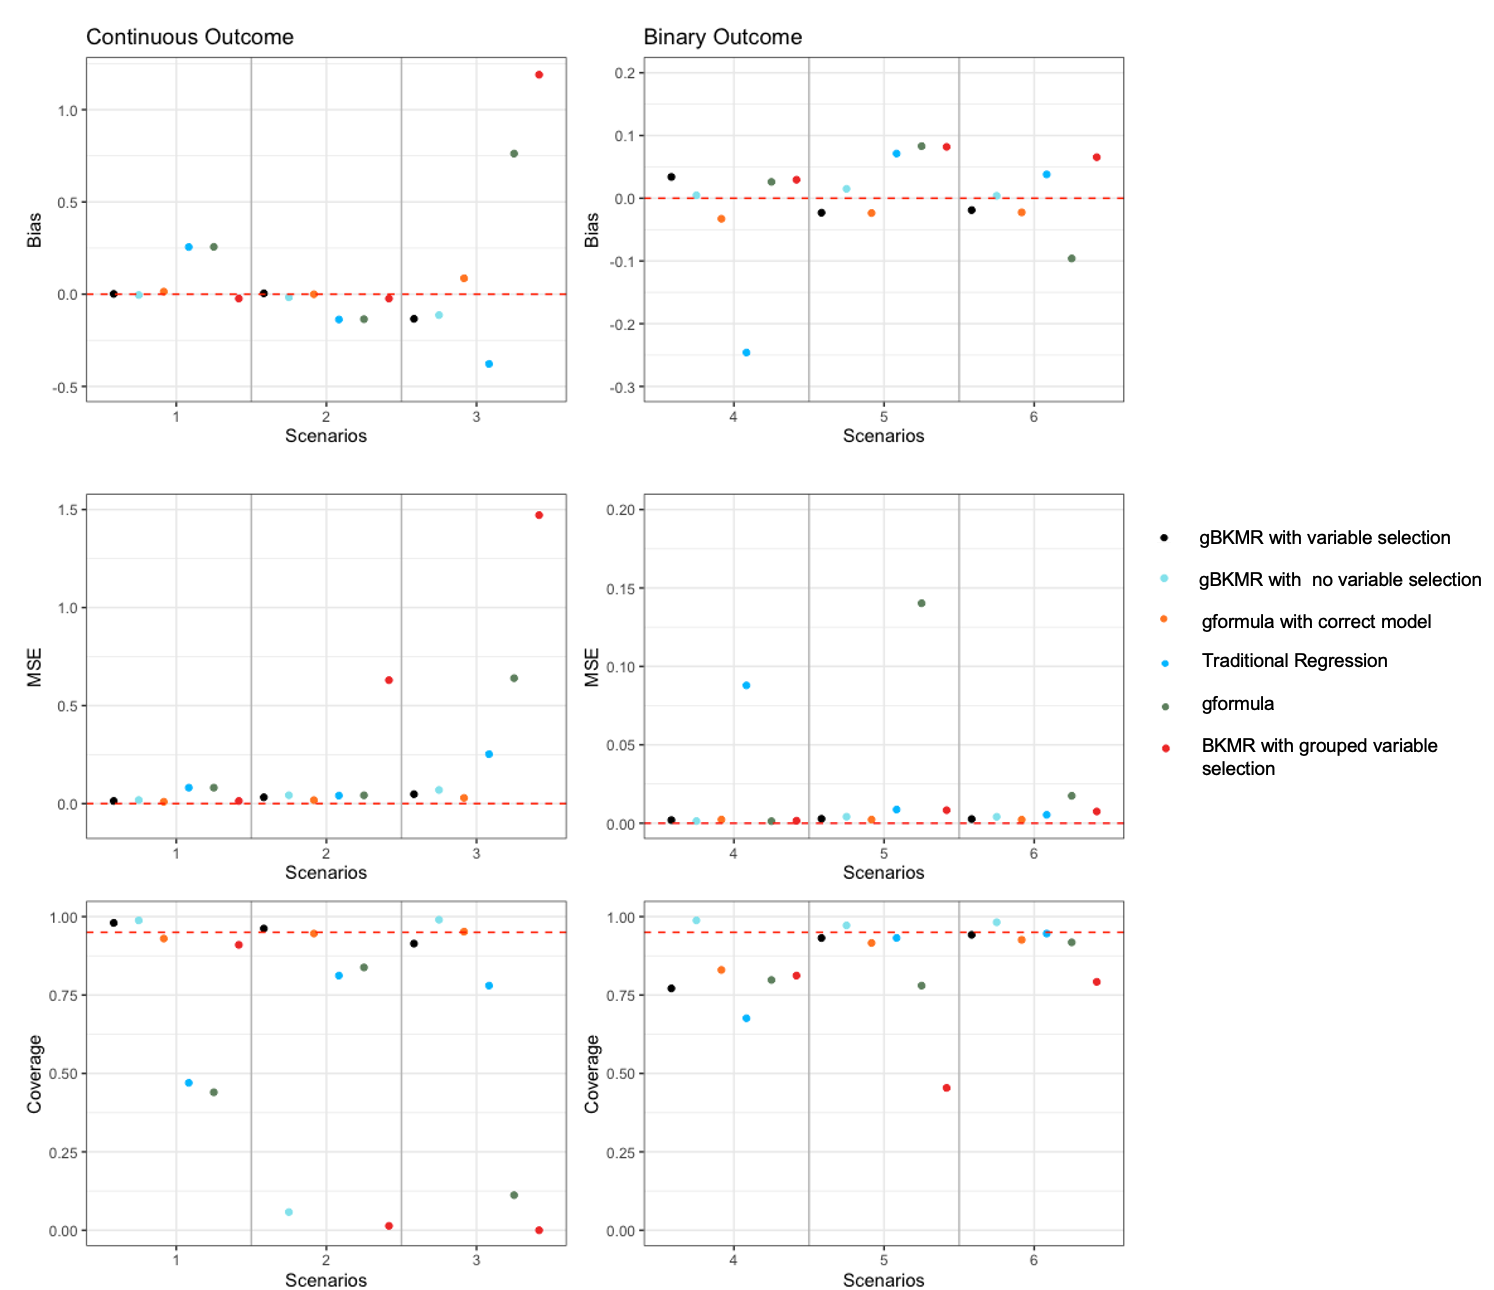
\includegraphics[width=0.95\textwidth]{figures/fig_simulation.png}
\caption{Bias, MSE, and coverage of the ATE estimates across the six simulation scenarios, comparing \pkg{CausalBKMR} (with and without variable selection) against the parametric g-formula, the parametric g-formula with correct model specification, traditional regression, and BKMR with grouped variable selection. Left column: continuous outcome (scenarios 1--3); right column: binary outcome (scenarios 4--6). Dashed red line indicates zero bias (top), zero MSE (middle), or nominal $95\%$ coverage (bottom).}
\label{fig:sim_results}
\end{figure}

\subsection*{Application to Strong Heart Study}

\subsubsection*{Study population and exposures}

We applied \pkg{CausalBKMR} to data from the Strong Heart Study \citep[SHS;][]{shs_lee_1990}, a prospective cohort of American Indian adults with low to moderate exposure to metals and a high burden of cardiometabolic disease. The analytic sample consisted of 679 participants with complete urinary metal measurements at three study visits (Visits 1--3) and fasting blood glucose measured at Visit 3. Six urinary metals were considered: selenium (Se), cadmium (Cd), molybdenum (Mo), tungsten (W), arsenic (As), and zinc (Zn), all standardised to urinary creatinine and log-transformed prior to analysis. The mixture comprised 18 exposure variables (six metals $\times$ three visits).

The outcome was log-transformed fasting blood glucose at Visit~3 (motivated by right-skewed distributions; skewness $1.8$--$2.1$). Time-varying confounders included waist circumference and fasting glucose measured at Visits 1 and 2, modeled as time-dependent covariates affected by prior exposure. Baseline covariates included age, sex, body mass index, study centre, smoking status (current/former/never), and baseline kidney function (CKD-EPI eGFR). Missing values were handled by multiple imputation ($m = 5$, predictive mean matching). The directed acyclic graph encoding the assumed causal structure is shown in Figure~\ref{fig:dag}; the cross-timepoint correlation matrix is shown in Figure~\ref{fig:corr}.

\subsubsection*{Model specification and estimation}

We denote the six-metal exposure vector at visit $t$ by $A_t = (A_{t,1}, \ldots, A_{t,6})$ for $t = 0, 1, 2$ (corresponding to Visits 1--3), the time-varying confounders at visit $t$ by $L_t = (\text{waist}_t, \text{glucose}_t)$ for $t = 1, 2$, the baseline covariates by $C_0$, and the outcome by $Y$ (log fasting glucose at Visit~3). Figure~\ref{fig:dag} shows the assumed causal structure: prior exposures $A_{<t}$ affect both current time-varying confounders $L_t$ and future exposures $A_t$, and all paths converge on $Y$. Note that $L_t$ are treated as time-varying confounders (not mediators): our goal is to recover the total causal effect of the exposure trajectory on $Y$ while accounting for the feedback between $A_t$ and $L_t$ over time, not to decompose it into direct and indirect pathways.

A key motivation for using \pkg{CausalBKMR} rather than a parametric g-formula is the extreme multicollinearity across metal-timepoint exposures (within-metal cross-visit correlations of $0.2$--$0.6$; Figure~\ref{fig:corr}). Fitting the g-formula with standard linear models in this setting yields unstable estimates with inflated standard errors, to the point that parametric g-computation did not produce interpretable results in preliminary analyses. \pkg{CausalBKMR} combines the flexibility of the Gaussian kernel with Bayesian regularisation, enabling valid inference under high correlation.

The \pkg{CausalBKMR} framework fits a sequence of BKMR models to implement the g-formula. At each visit $t \in \{1, 2\}$, separate models for the time-varying confounders were fit for waist circumference and fasting glucose, each regressing on all prior exposures and confounder values through a Gaussian kernel, with $C_0$ entering parametrically. An outcome model for Visit~3 log glucose was then fit on the full exposure and confounder history. All models used component-wise variable selection \citep{bobb_bkmr_2015} and were fit with $24{,}000$ MCMC iterations using 50 knots. All exposures and time-varying confounders were standardised to zero mean and unit variance before entering the kernel. Visit~3 waist and glucose values in the outcome model were imputed via last-observation-carried-forward, since Visit~3 glucose is the outcome itself.

We enabled component-wise variable selection in all BKMR models because it serves two purposes in this application: (i) it regularises the high-dimensional kernel against the strong within-metal temporal correlation and (ii) the spike-and-slab prior automatically accounts for multiple testing across the 18 exposure variables, yielding valid Bayesian inference for the components that are selected---a property not shared by frequentist regularisation methods such as the lasso. As a consequence, exposures with near-zero posterior inclusion probability are shrunk to zero and the corresponding credible intervals collapse; these should be read as ``no evidence of association,'' not as missing estimates.

Causal effects were estimated via Monte Carlo g-computation over 40 retained posterior draws (iterations $22{,}000$--$24{,}000$, every 50th). For each draw, $K = 1{,}000$ counterfactual trajectories were simulated under two static exposure regimes: $\mathbf{a}$ (all exposures at their 25th percentile) and $\mathbf{a}^*$ (all at a target percentile $q$). Counterfactual values of $L_t$ were sampled sequentially forward in time---first $L_1$ given $A_0$, then $L_2$ given $(A_0, A_1, L_1)$---and the outcome was predicted conditional on the full counterfactual history. The average causal effect at each $q$ was computed as the posterior mean difference $E[Y_{\mathbf{a}^*}] - E[Y_{\mathbf{a}}]$, with 95\% credible intervals from the 2.5th and 97.5th percentiles pooled across all five imputed datasets.

We targeted two estimands: (i) the joint mixture causal effect for $q \in \{0.30, 0.35, \ldots, 0.90\}$, yielding a causal dose-response curve, and (ii) single-variable causal effects, shifting one metal at one visit from its 25th to 75th percentile while holding all others at their median.

\subsubsection*{Application results}

Before interpreting the causal effect estimates, we inspected MCMC trace plots for all BKMR models and confirmed good mixing and convergence across chains for each imputed dataset. We additionally verified that conclusions were qualitatively unchanged under alternative prior specifications for the kernel smoothness parameter, supporting the robustness of posterior inference.

The joint mixture causal effect on log fasting glucose followed a positive, approximately monotonic dose-response (Figure~\ref{fig:dr-joint}). The 95\% credible interval excluded zero above approximately the 45th percentile, with the magnitude of the effect increasing through the upper end of the exposure distribution. At the 75th vs.\ 25th percentile contrast, the average causal effect was $1.01$ standardised units of log glucose (95\% CrI: $0.72$, $1.33$). Examining each metal-timepoint individually (Figure~\ref{fig:forest}), zinc was the dominant contributor to the joint mixture signal: the IQR causal effect of Zn was $0.51$ SD at Visit~1 (95\% CrI: $0.28$, $0.75$), $0.26$ SD at Visit~2 ($0.03$, $0.51$), and $0.36$ SD at Visit~3 ($0.20$, $0.55$). All three Zn-timepoint effects were credibly distinct from zero. Selenium at Visit~1 also showed a positive association ($0.19$ SD; 95\% CrI: $-0.01$, $0.36$; posterior probability of a positive effect: $0.97$). Cadmium at Visit~1 showed an inverse association ($-0.21$ SD; 95\% CrI: $-0.37$, $-0.05$). Several metal-timepoints (Mo, W, As, and the later visits of Se and Cd) had point estimates and credible intervals concentrated at zero: these components were not selected by the spike-and-slab prior in any retained MCMC iteration and should be interpreted as providing no evidence of an association, rather than as having zero-width intervals.

\subsubsection*{Sensitivity analyses}

We conducted two sensitivity analyses to assess the robustness of the main findings. First, to evaluate whether the metal--glucose associations were driven by participants with established diabetes, we excluded the 265 participants with baseline diabetes (WHO clinical definition; analytic sample $n = 414$). In this subsample, the joint mixture dose-response was substantially attenuated, with the 95\% credible interval covering zero across most quantile contrasts (Figure~\ref{fig:dr-compare}). Single-variable effects were also markedly reduced: Zn(V1) decreased from $0.51$ to $0.01$ SD, Cd(V1) reversed sign and became non-significant, and most other estimates moved toward the null. Two findings remained robust: Se(V1) remained positive and credibly above zero ($0.07$ SD; 95\% CrI: $0.004$, $0.15$), and Zn(V3) retained a borderline positive signal ($0.14$ SD; 95\% CrI: $0.00$, $0.35$).

Second, to address potential residual confounding by smoking intensity---particularly relevant to the inverse Cd(V1) finding---we additionally adjusted for baseline pack-years alongside the categorical smoking-status variable. For never-smokers, pack-years was set to zero prior to multiple imputation. All findings were robust to this adjustment: the joint dose-response at the 75th vs.\ 25th percentile was $1.06$ SD (95\% CrI: $0.80$, $1.39$), compared with $1.01$ ($0.72$, $1.33$) in the main analysis. Notably, the inverse Cd(V1) effect was essentially unchanged ($-0.22$ SD; 95\% CrI: $-0.35$, $-0.10$), indicating that this association is not explained by smoking intensity alone.

\begin{figure}[h]
\centering
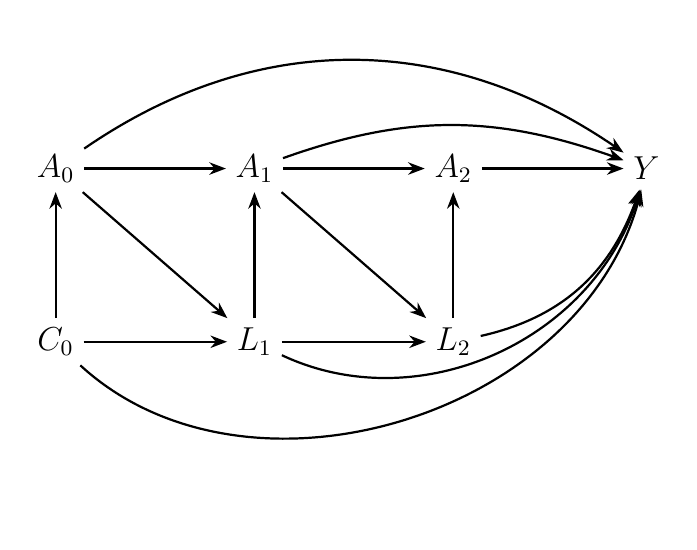
\begin{tikzpicture}[
    node distance=1.6cm and 1.8cm,
    every node/.style={font=\large},
    arr/.style={-{Stealth[length=6pt]}, thick}
]
\node (A0) {$A_0$};
\node (A1) [right=of A0] {$A_1$};
\node (A2) [right=of A1] {$A_2$};
\node (Y)  [right=of A2] {$Y$};
\node (C0) [below=of A0] {$C_0$};
\node (L1) [below=of A1] {$L_1$};
\node (L2) [below=of A2] {$L_2$};
\draw[arr] (A0) -- (A1);
\draw[arr] (A1) -- (A2);
\draw[arr] (A2) -- (Y);
\draw[arr] (C0) -- (L1);
\draw[arr] (L1) -- (L2);
\draw[arr] (C0) -- (A0);
\draw[arr] (L1) -- (A1);
\draw[arr] (L2) -- (A2);
\draw[arr] (A0) -- (L1);
\draw[arr] (A1) -- (L2);
\draw[arr, bend left=35]  (A0) to (Y);
\draw[arr, bend left=20]  (A1) to (Y);
\draw[arr, bend right=60] (C0) to (Y);
\draw[arr, bend right=50] (L1) to (Y);
\draw[arr, bend right=30] (L2) to (Y);
\end{tikzpicture}
\caption{Directed acyclic graph showing time-varying exposures ($A_t$), time-varying confounders ($L_t$), baseline covariates ($C_0$), and outcome ($Y$) at 3 visits.}
\label{fig:dag}
\end{figure}

\begin{figure}[h]
\centering
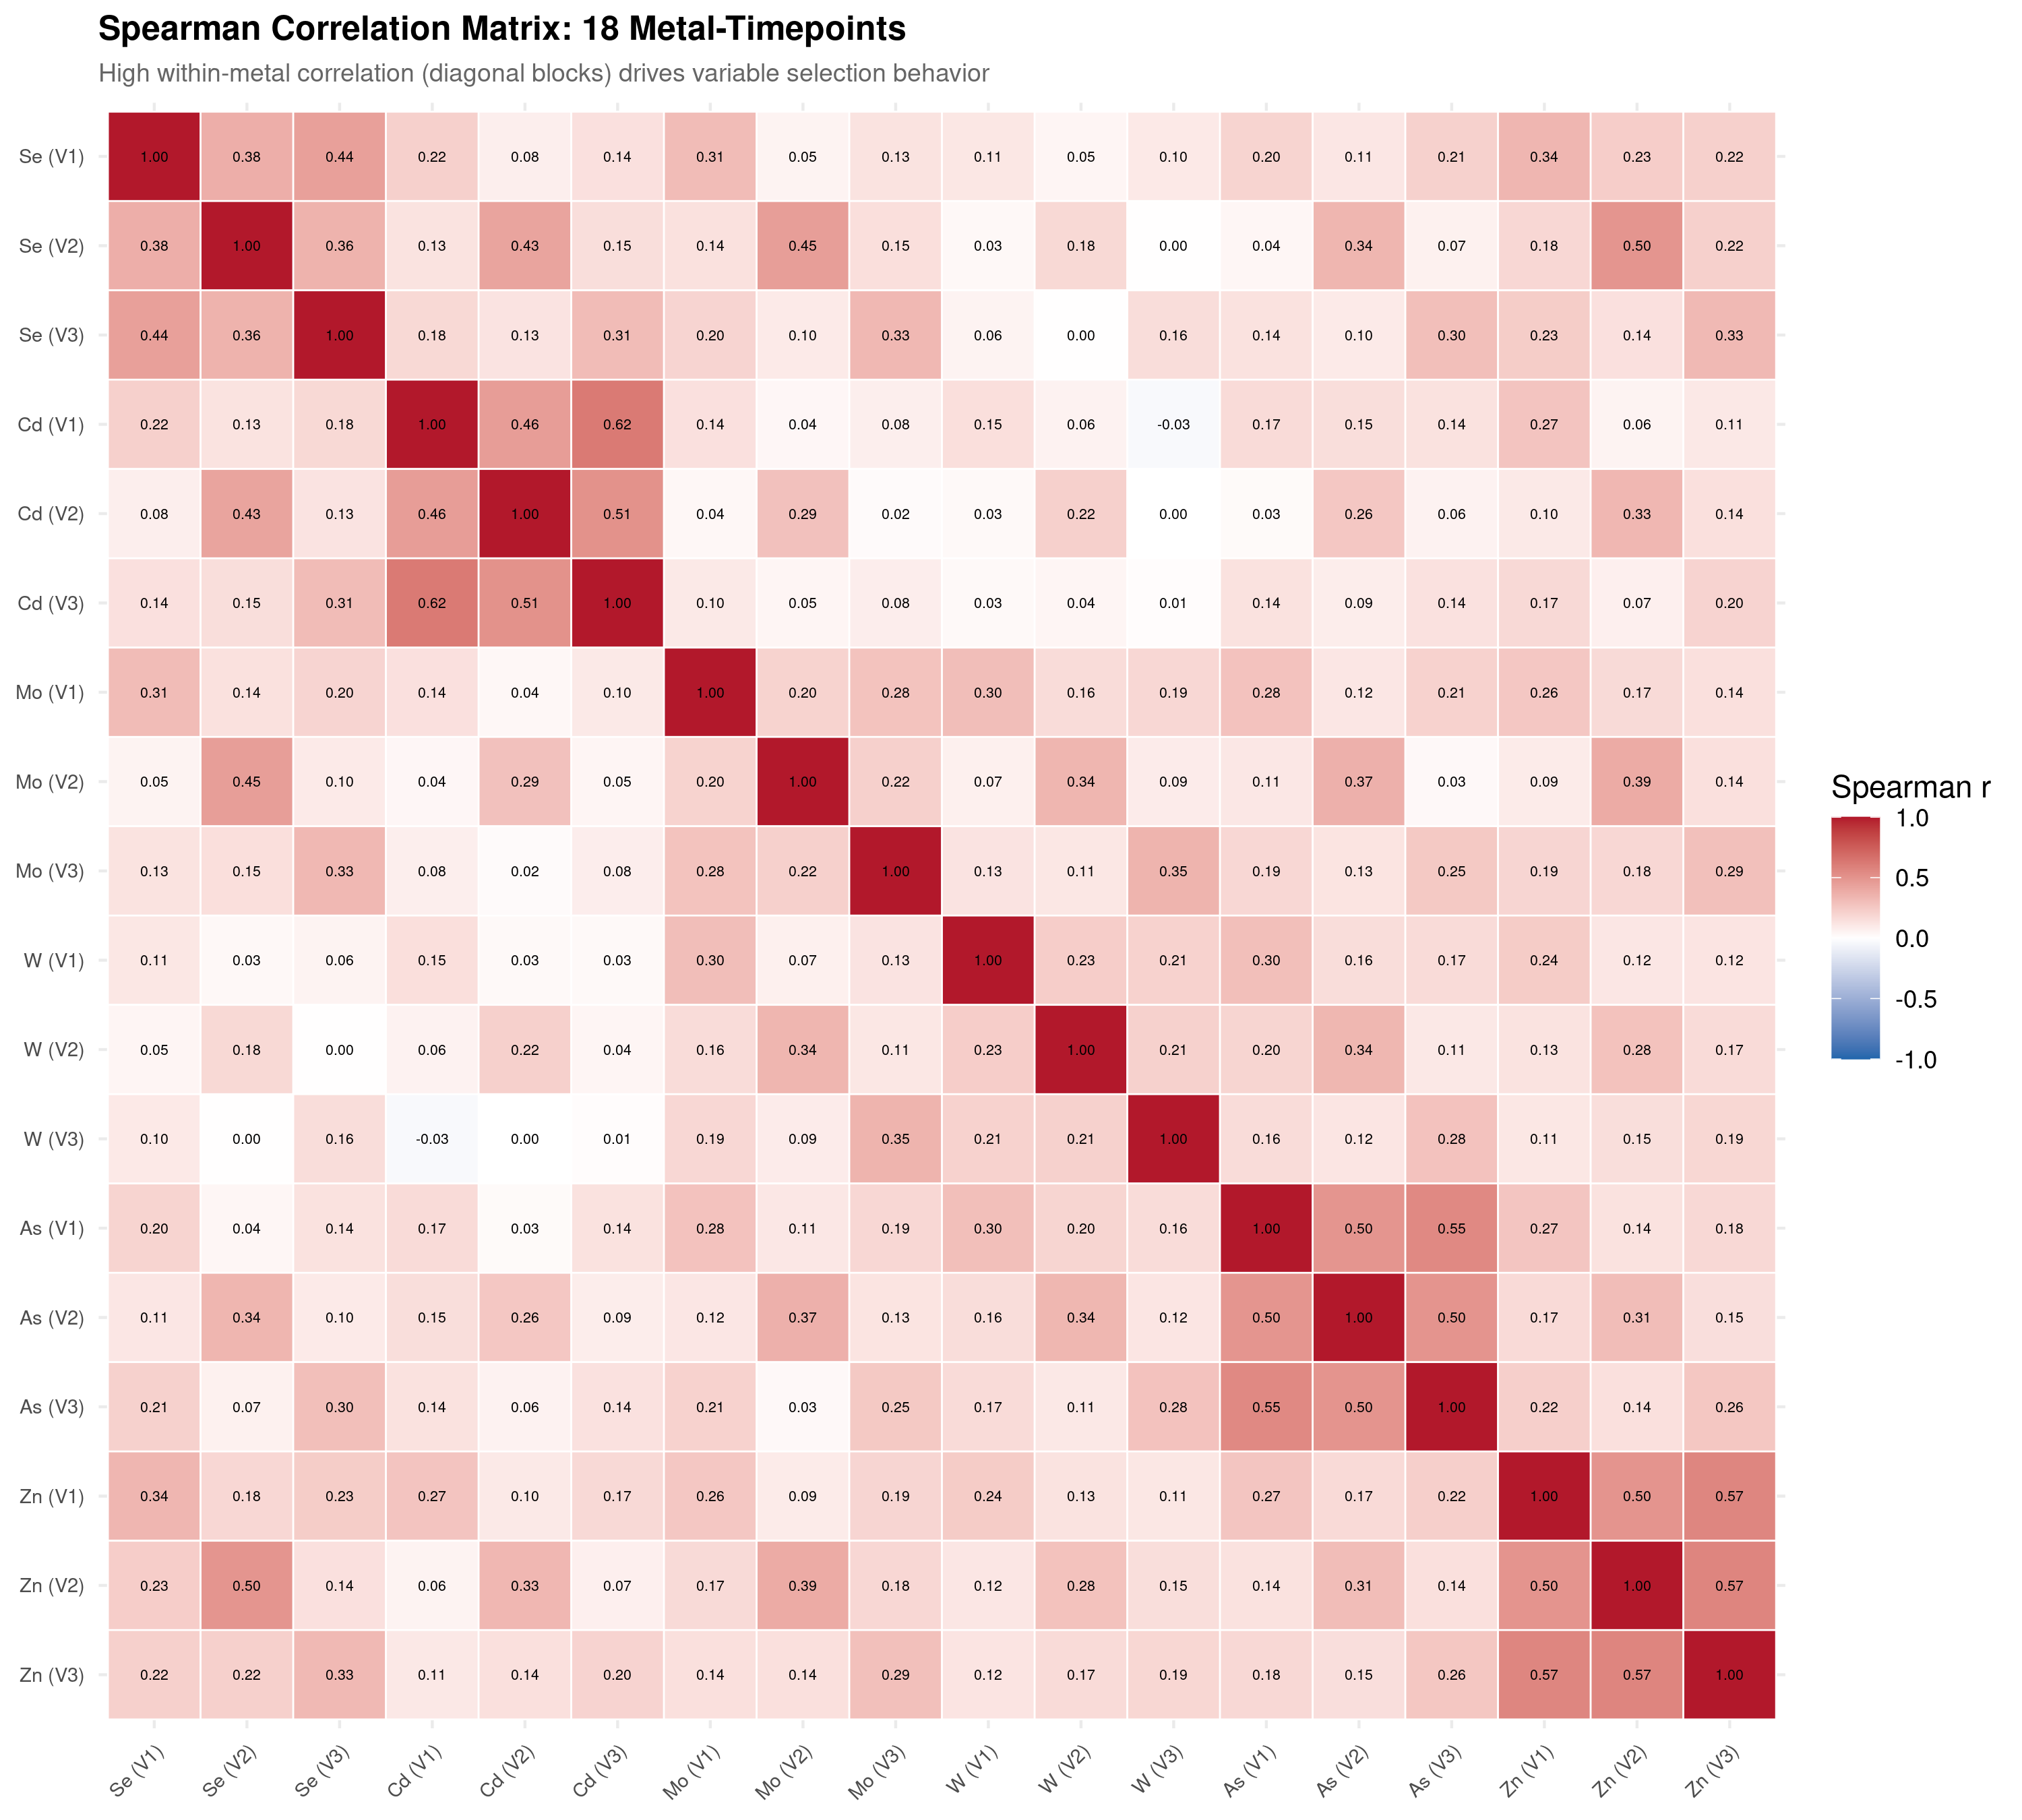
\includegraphics[width=0.85\textwidth]{figures/fig_cross_timepoint_corr_matrix.png}
\caption{Spearman correlation matrix of the 18 metal-timepoint exposures (six metals $\times$ three visits).}
\label{fig:corr}
\end{figure}

\begin{figure}[h]
\centering
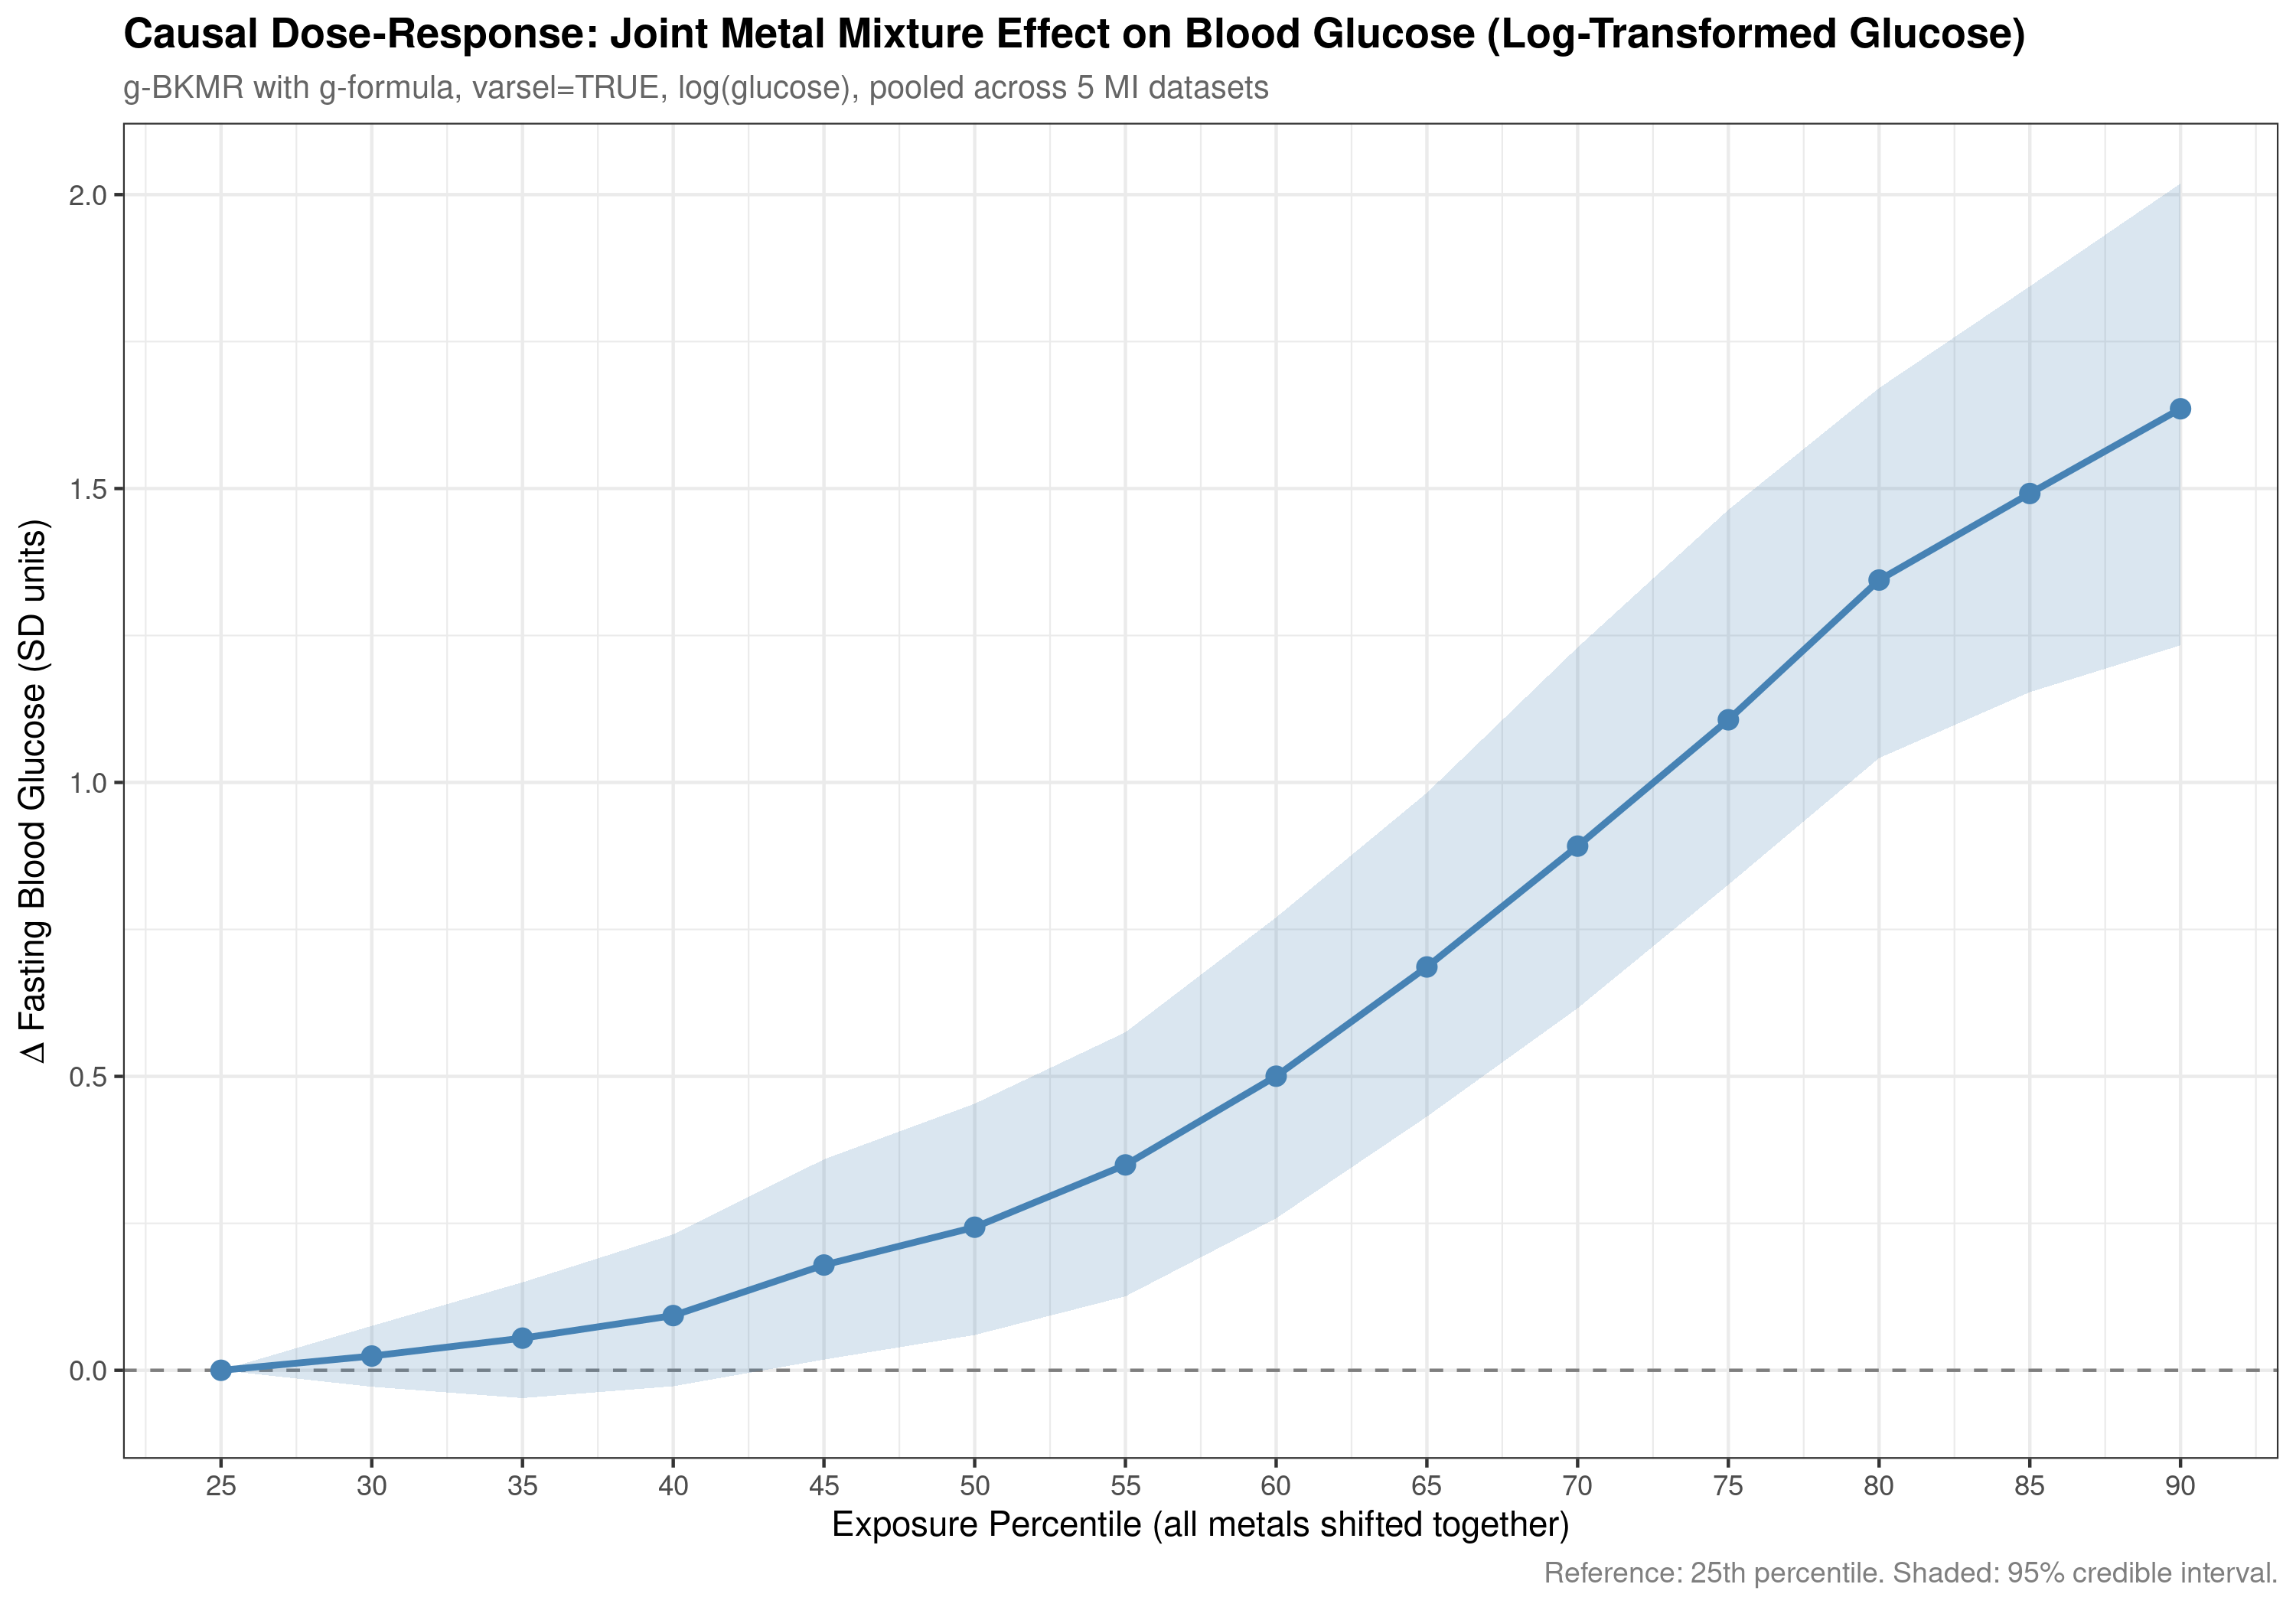
\includegraphics[width=0.85\textwidth]{figures/fig_dr_full.png}
\caption{Joint causal dose-response of the metal mixture on log fasting glucose, full sample ($n = 679$). Reference: 25th percentile. Shaded band: 95\% credible interval.}
\label{fig:dr-joint}
\end{figure}

\begin{figure}[h]
\centering
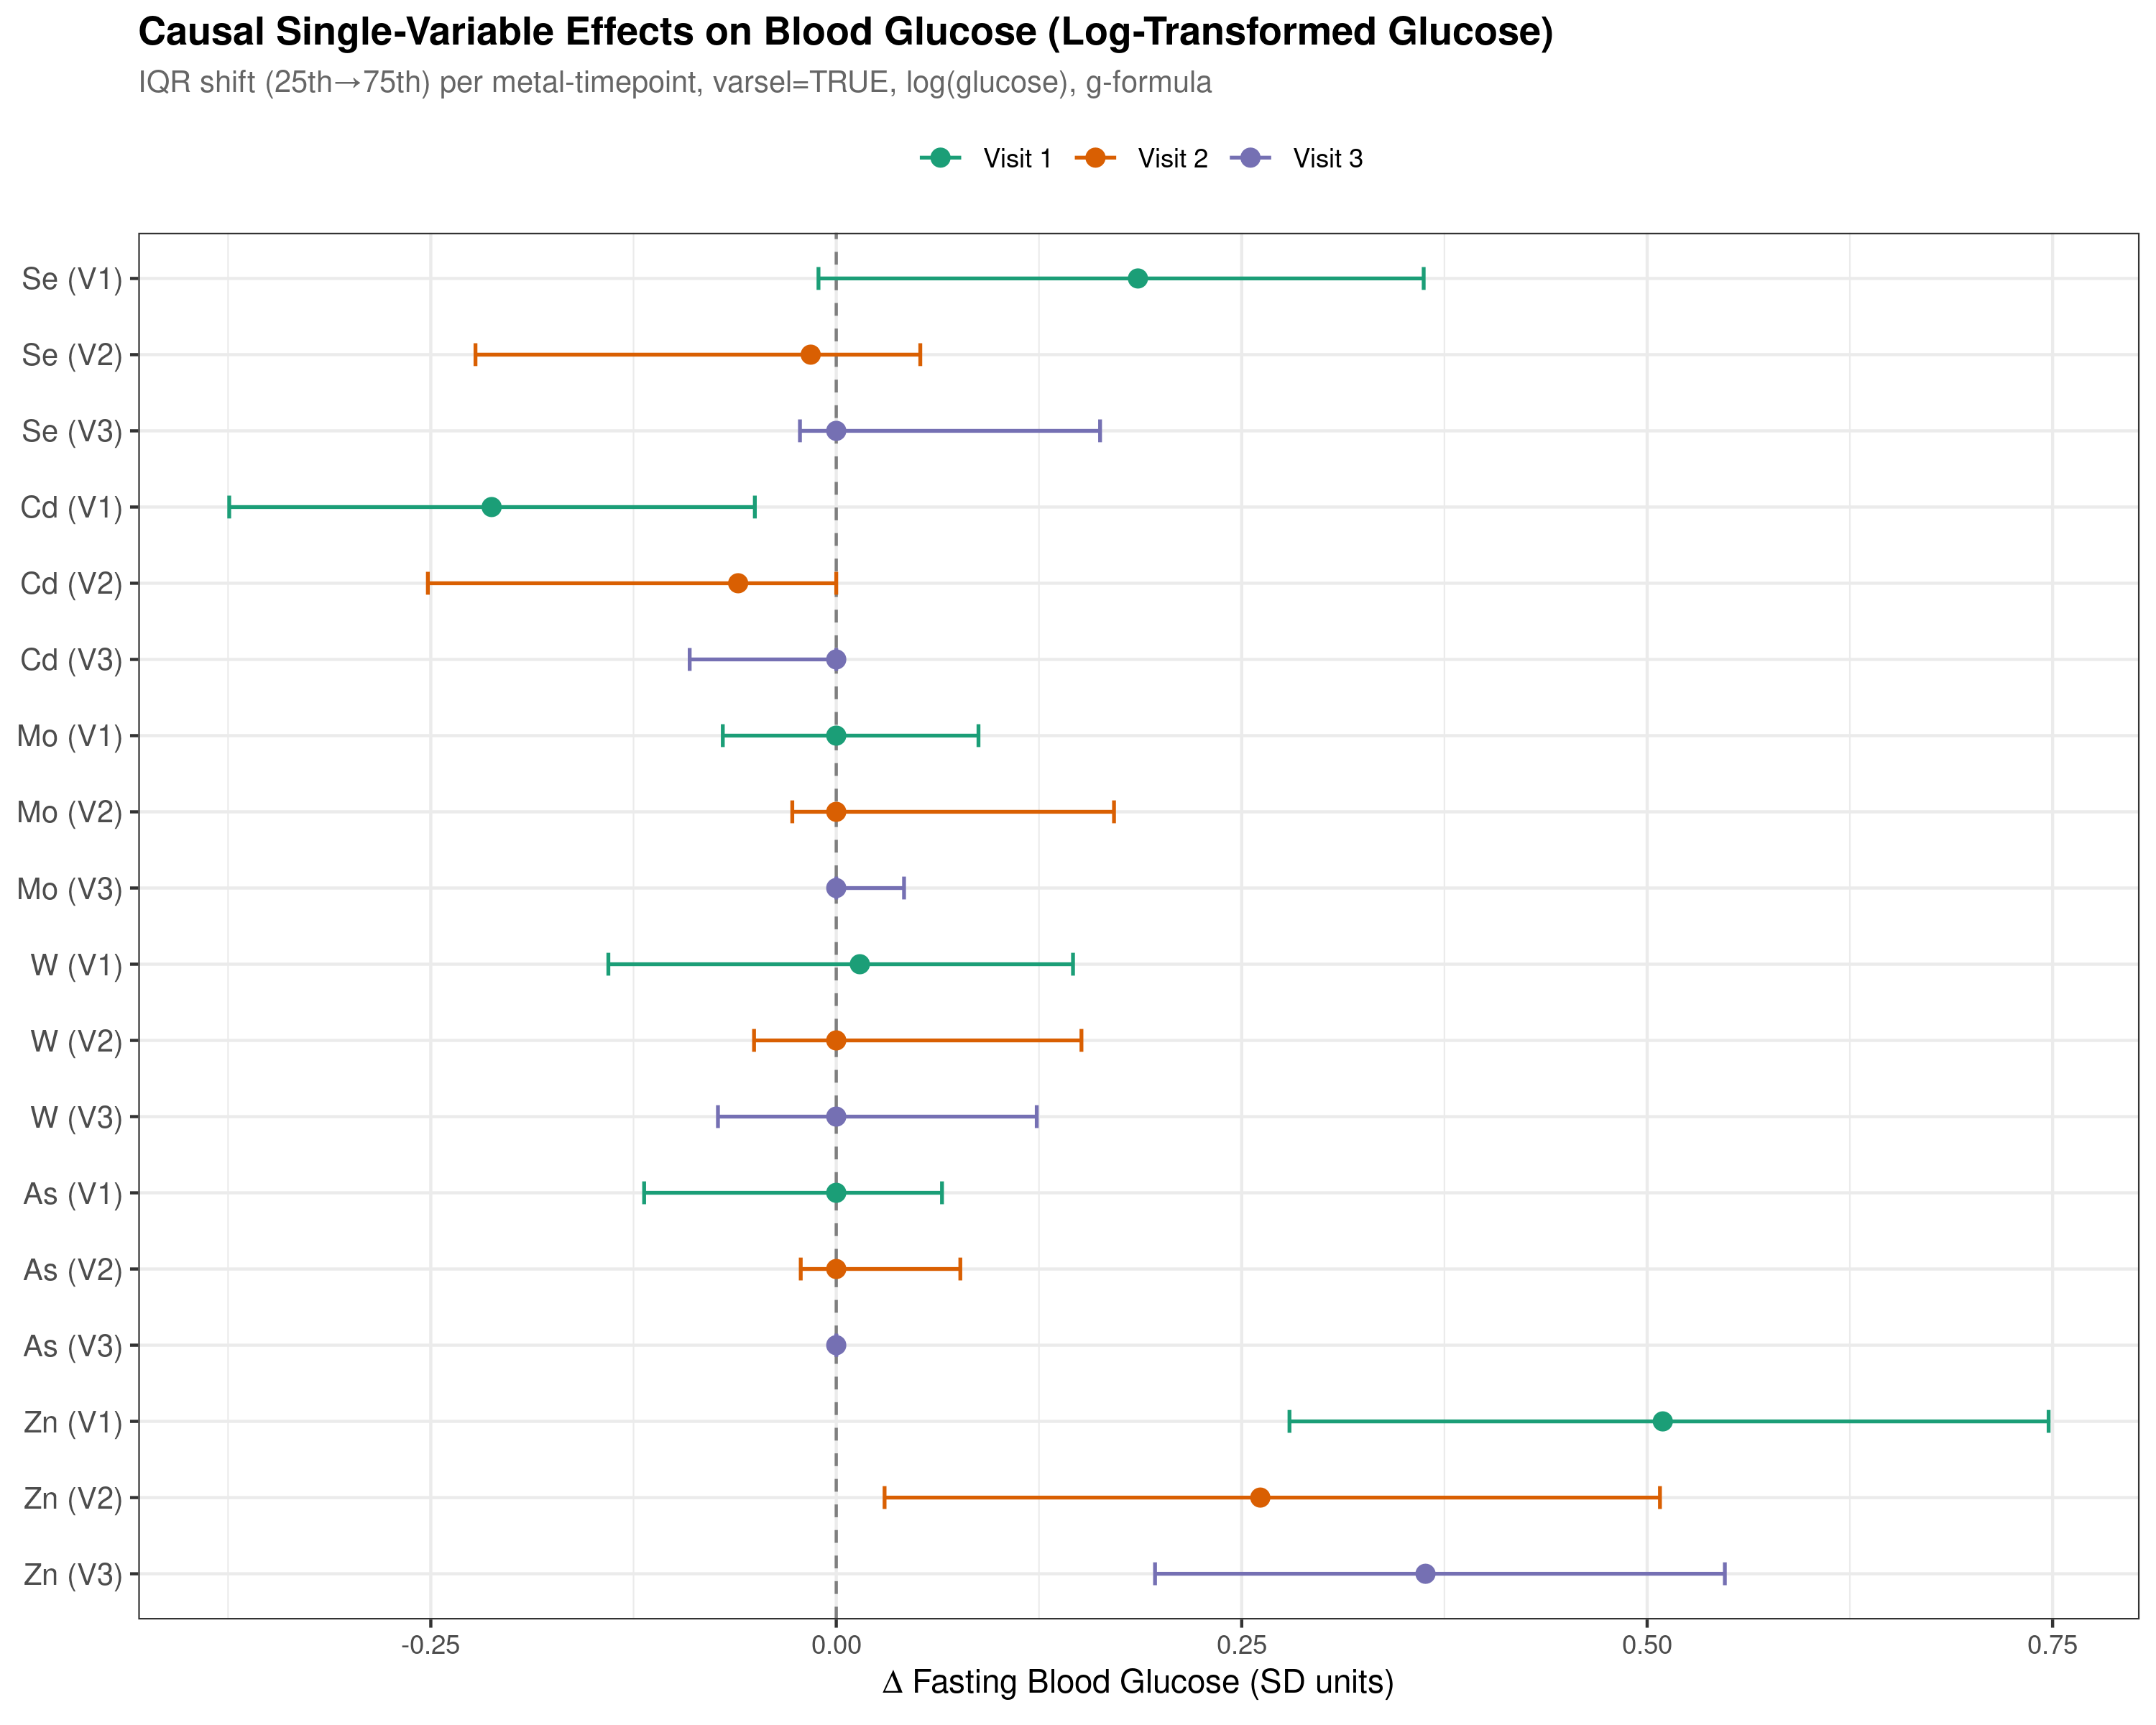
\includegraphics[width=0.85\textwidth]{figures/fig_forest_full.png}
\caption{Single-variable causal effects (IQR shift, 25th to 75th percentile). Bars: 95\% credible intervals. Full sample, $n = 679$.}
\label{fig:forest}
\end{figure}

\begin{figure}[h]
\centering
\begin{subfigure}{0.48\textwidth}
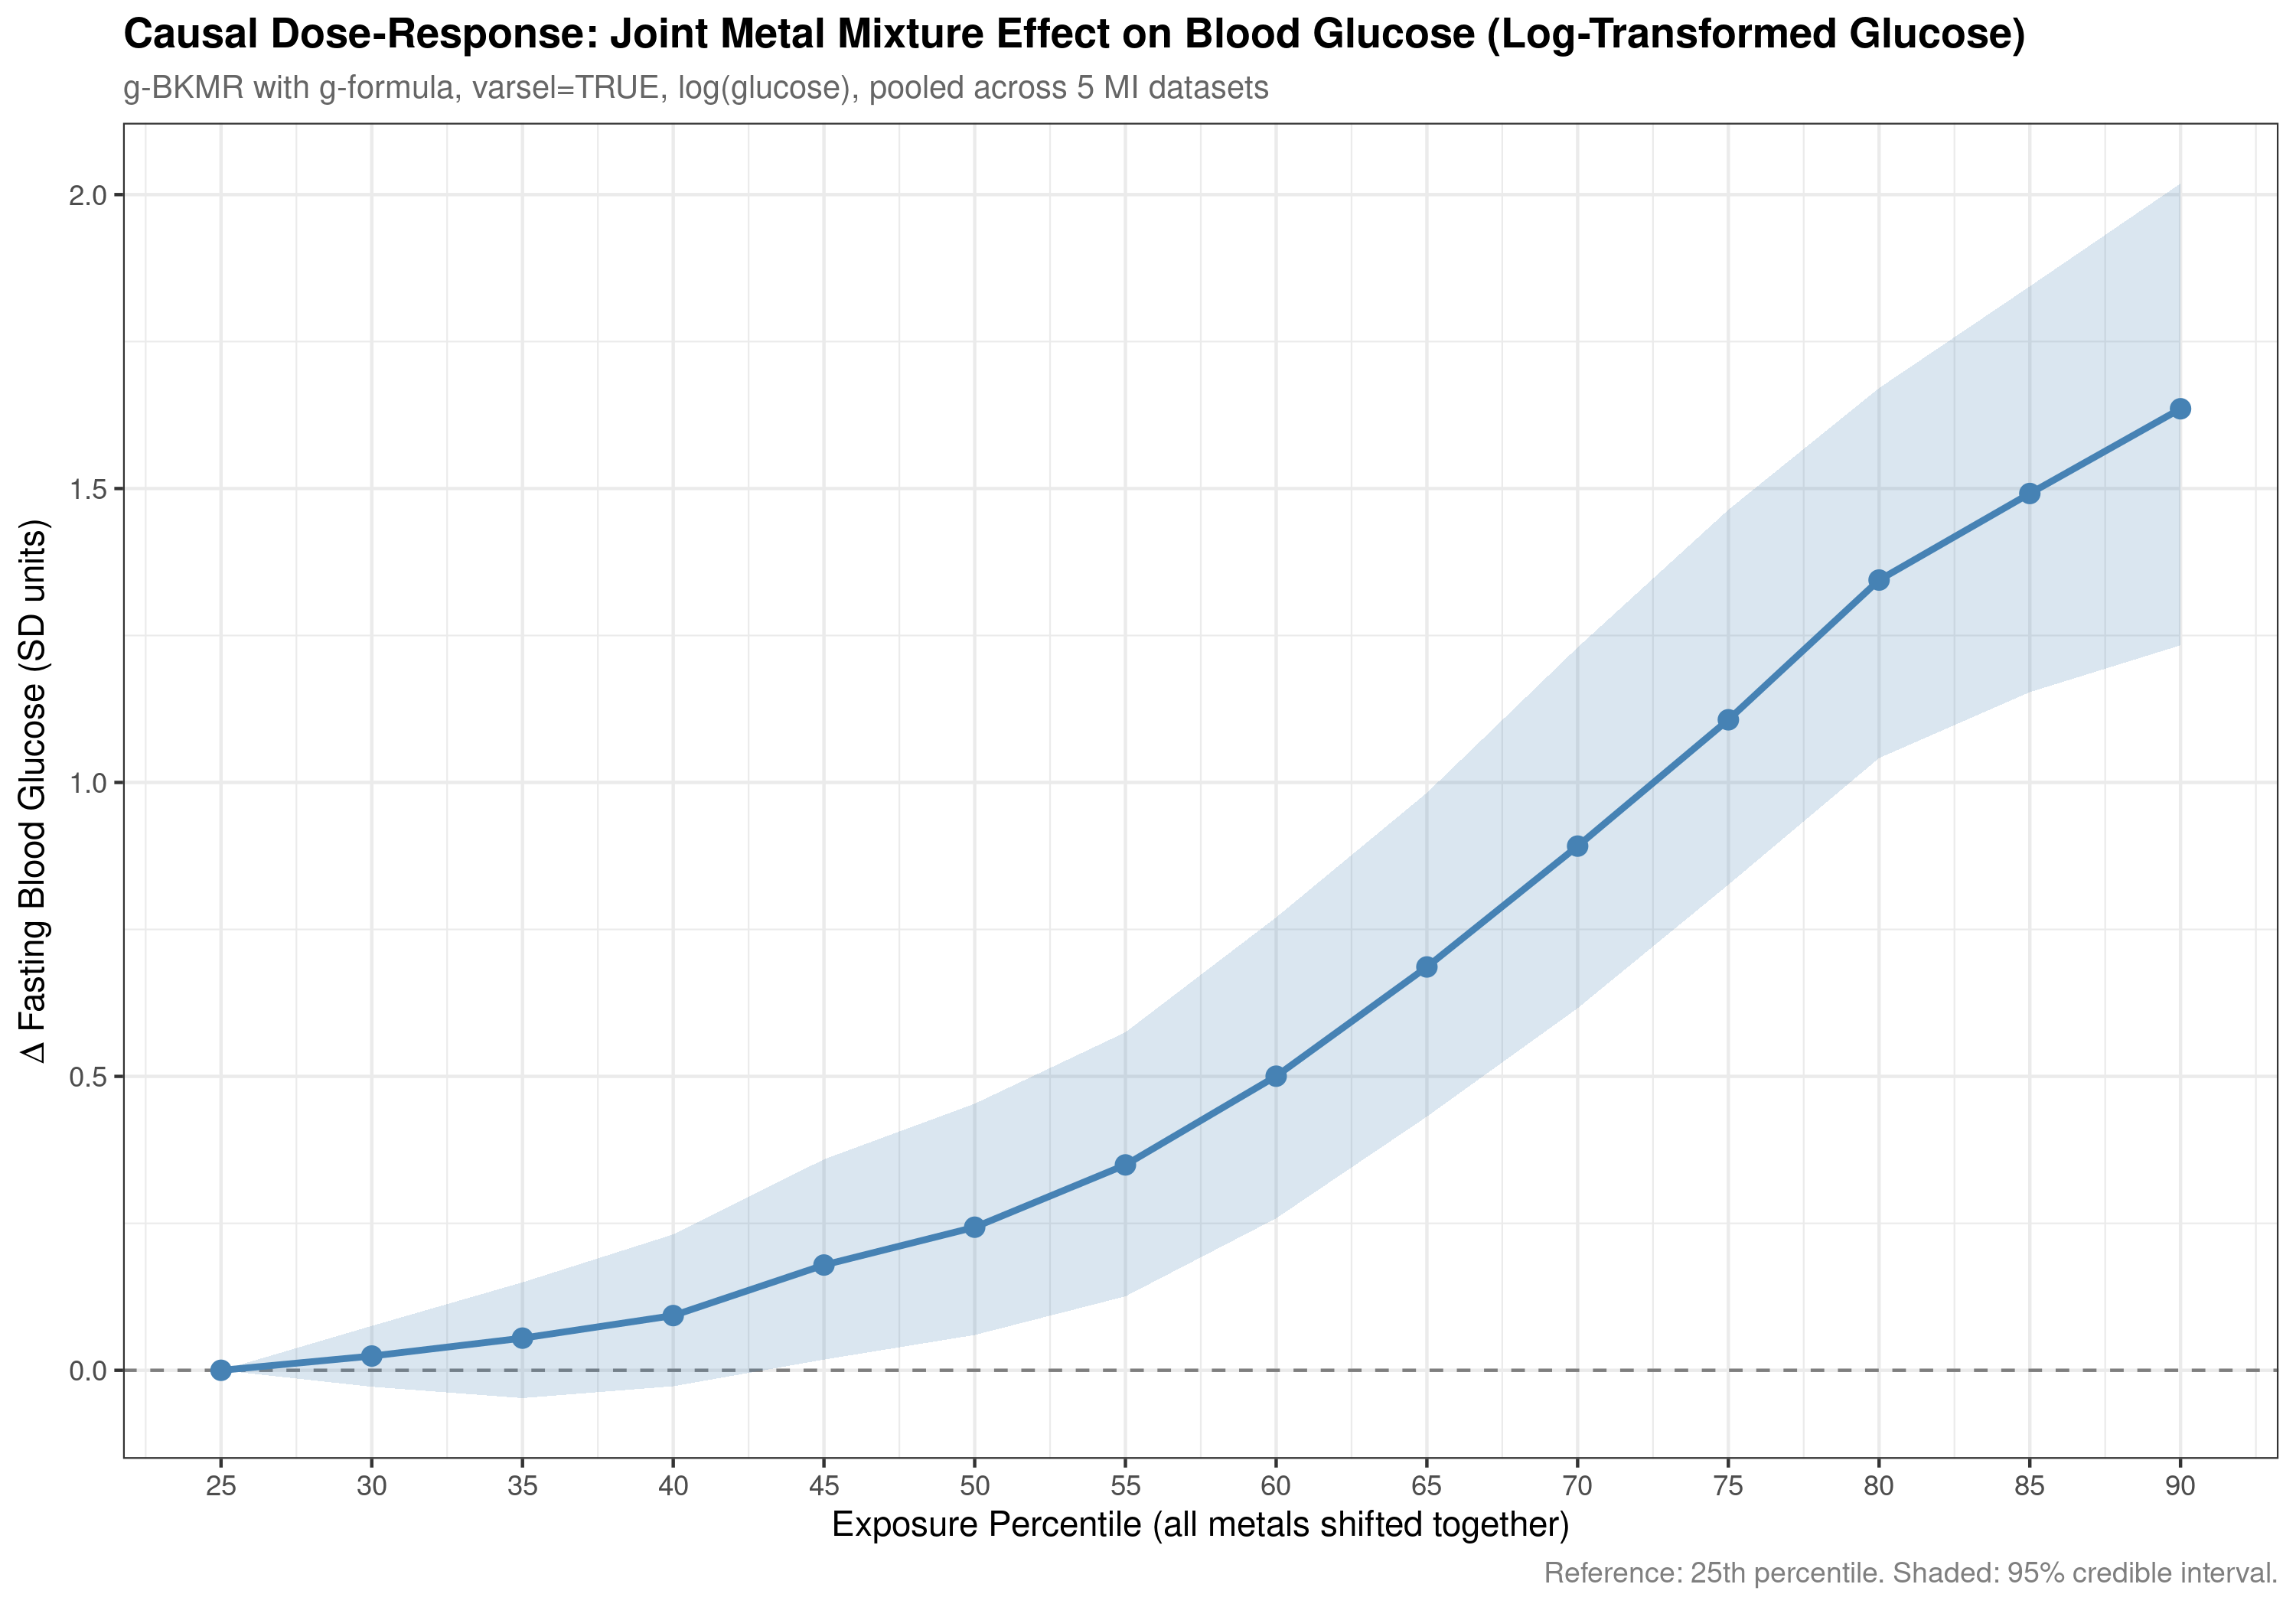
\includegraphics[width=\textwidth]{figures/fig_dr_full.png}
\caption{Full sample ($n = 679$)}
\end{subfigure}\hfill
\begin{subfigure}{0.48\textwidth}
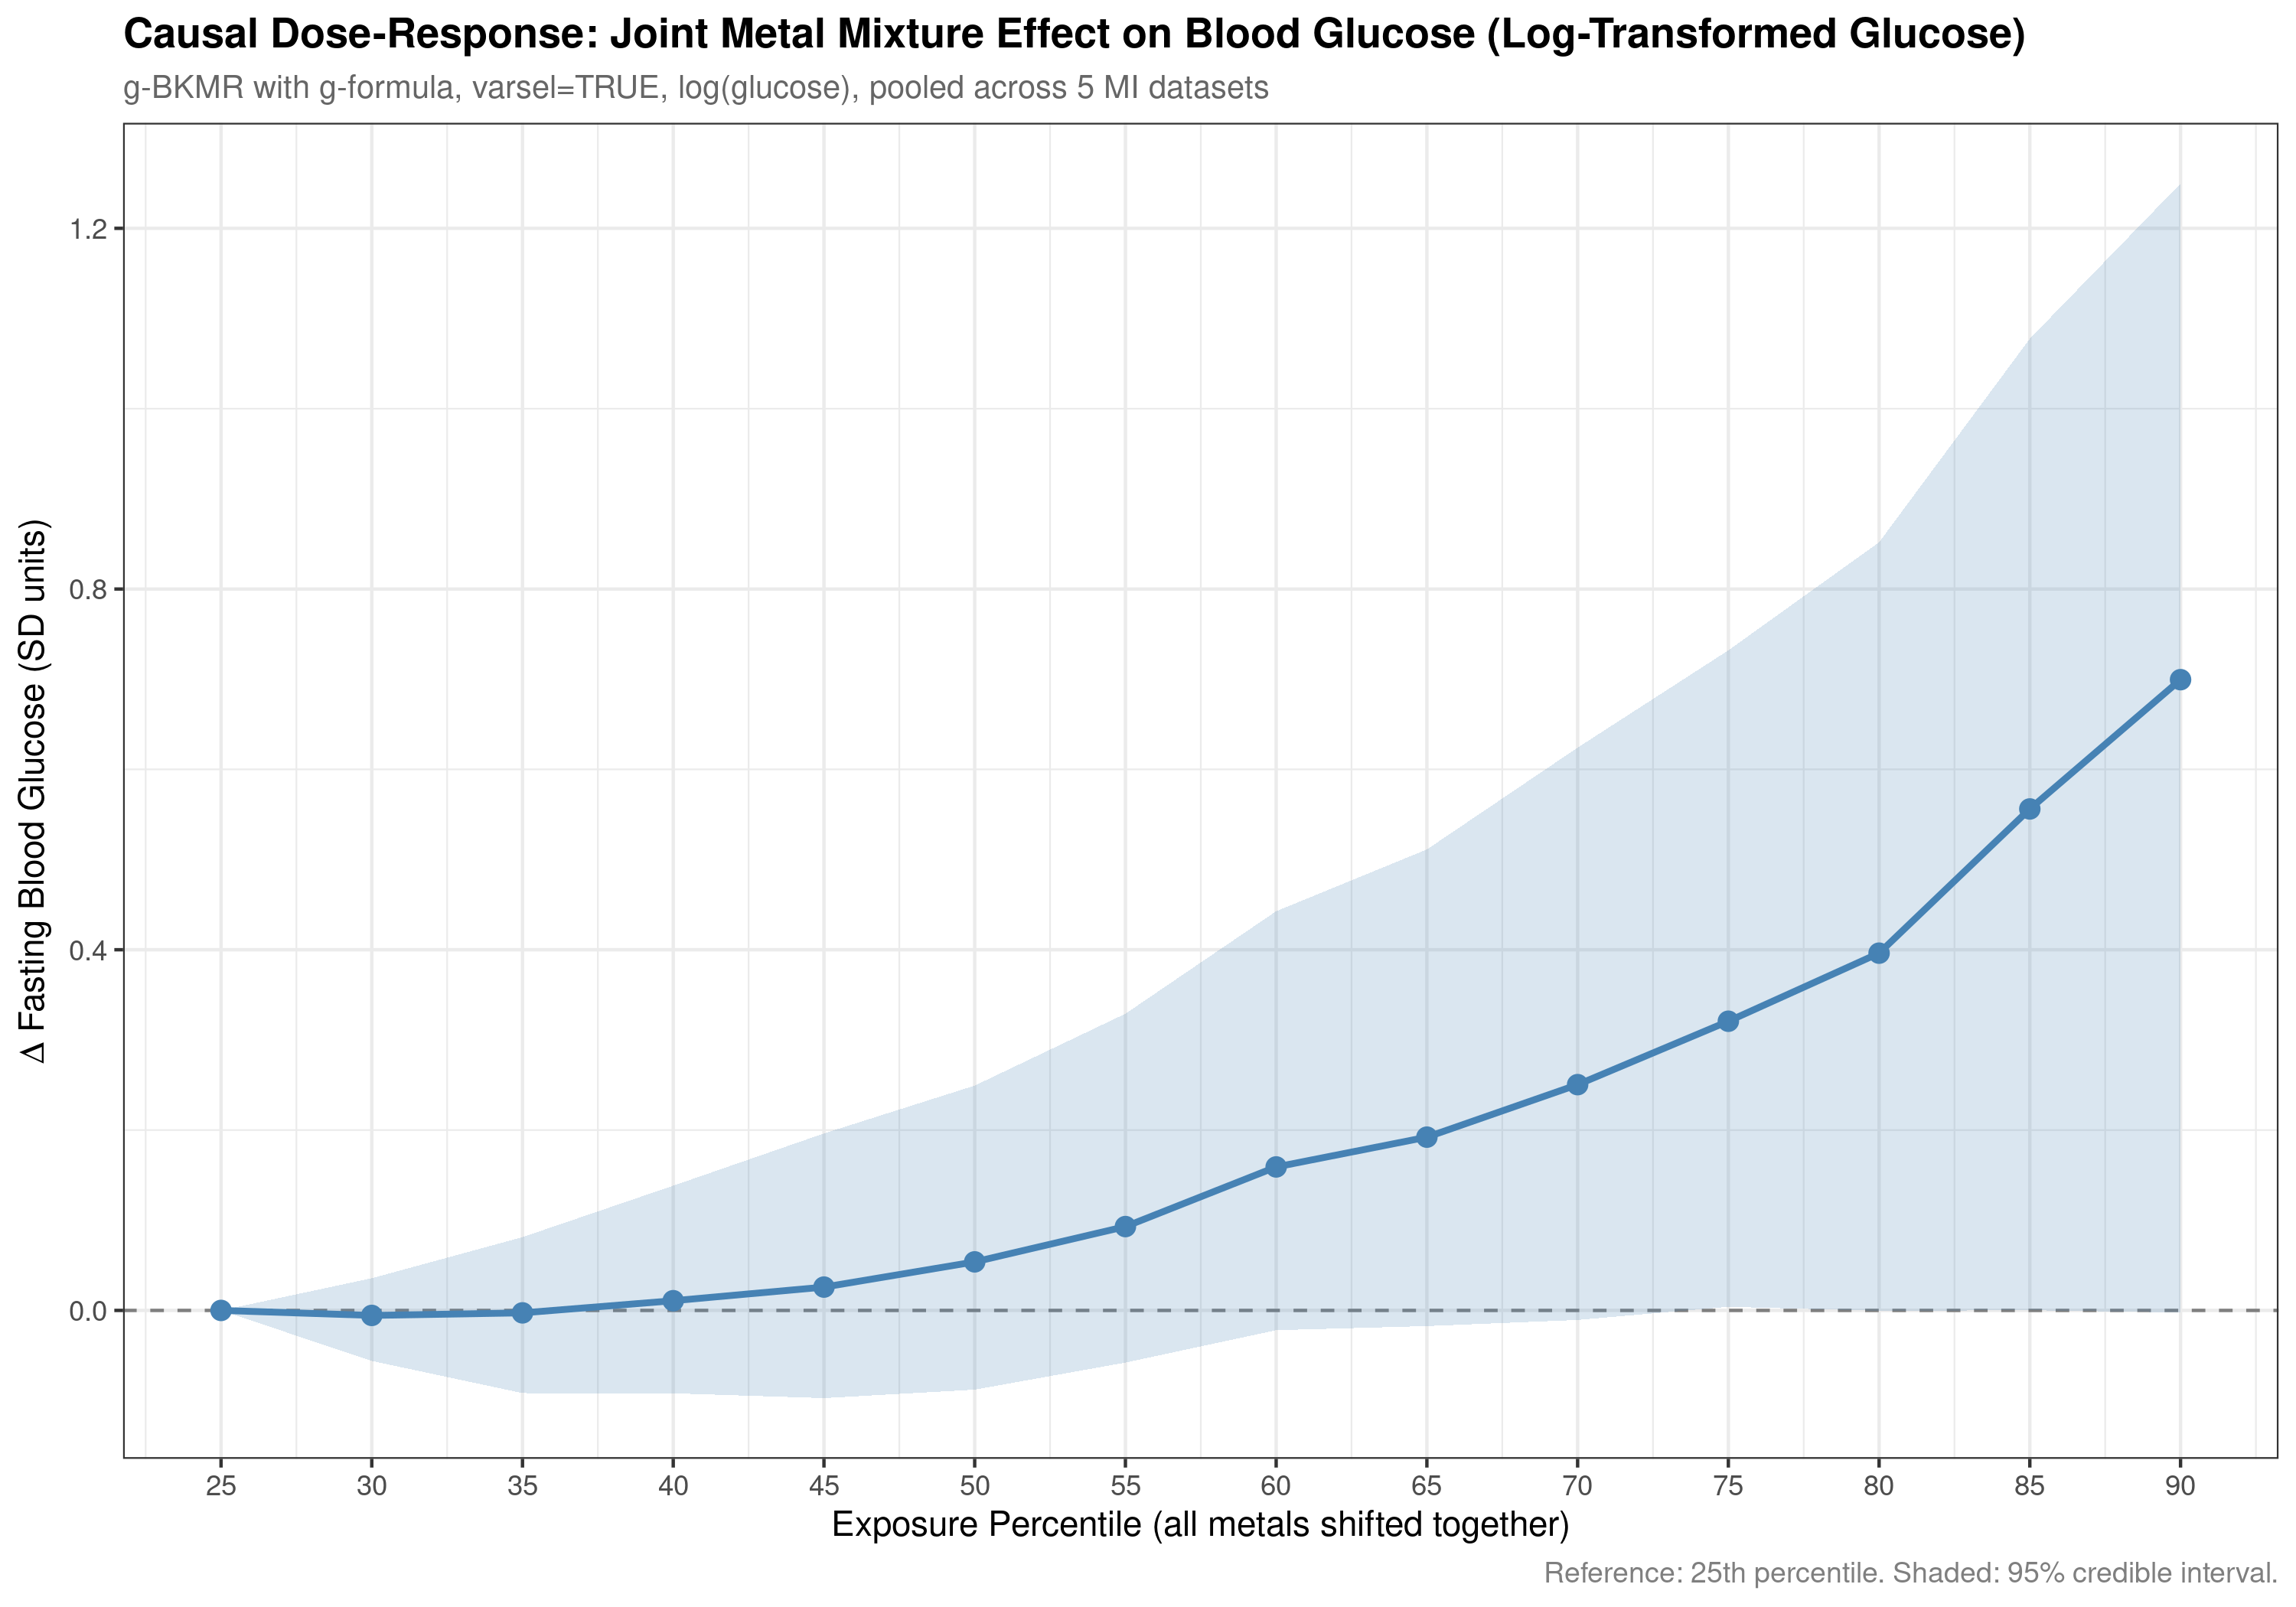
\includegraphics[width=\textwidth]{figures/fig_dr_nodm.png}
\caption{Excluding baseline diabetes ($n = 414$)}
\end{subfigure}
\caption{Sensitivity: joint dose-response in full sample (left) vs.\ excluding baseline diabetes (right).}
\label{fig:dr-compare}
\end{figure}

\subsection*{fastBKMR computational benchmark}

Standard BKMR scales poorly with cohort size because the Gaussian kernel requires $O(n^3)$ operations per MCMC iteration, which limits applicability of the standard \pkg{bkmr} engine in modern cohorts. The optional \code{engine = "fastbkmr"} path in \pkg{CausalBKMR} addresses this by calling \pkg{fbkmr} \citep{sonabend_fastbkmr_2026}, which fits the Bayesian kernel machine regression on multiple data subsets in parallel and recombines posterior draws through median-posterior subset aggregation. To document the practical computational gains and validate the subset approximation, we benchmarked the fastBKMR engine against the standard \pkg{bkmr} engine on a longitudinal data-generating mechanism matching the Strong Heart Study application in structure ($T=3$ visits, $p=4$ exposures per visit, one time-varying confounder, continuous outcome, $\alpha_1 = 0.6$) but scaled to MESA-cohort sample sizes ($n = 6{,}000$). The continuous-outcome DGP is the supported configuration of \code{engine = "fastbkmr"} per Table~\ref{tab:engine_support}; we additionally verified that the wall-clock characteristics are insensitive to outcome family by re-running the same fitting code under a binary-outcome DGP (Scenario 3c), with negligible difference because \code{kmbayes()} and \code{skmbayes()} both fit Gaussian kernel regressions on $y$ regardless of how $y$ was generated.

For each of three model types in the g-formula sequence (mediator at $t=1$ with 4 kernel inputs, mediator at $t=2$ with 9 inputs, and outcome model with 14 inputs), we fit three configurations: (i) standard BKMR with $n = 500$ random subsample and 50 knots; (ii) standard BKMR with $n = 2{,}000$ random subsample and 50 knots; and (iii) fastBKMR on the full $n = 6{,}000$ sample using 10 random subsets of size $\sim 600$, fit in parallel on 10 cores via \code{skmbayes(parallel = TRUE)}. Each configuration was replicated three times. The standard BKMR runs used 15{,}000 MCMC iterations; the fastBKMR runs used 1{,}000 iterations per subset and set \code{est.h = FALSE} so that the spatial smoothing variance is estimated post hoc rather than at each iteration. Two baseline covariates (sex and waist circumference at baseline) entered each model linearly. Knot approximation is not currently supported in \code{skmbayes()}.

Table~\ref{tab:fastbkmr_time} reports per-model wall-clock time across the three methods. \todo{The numbers below are pending the controlled continuous-outcome rerun (Scenario 3d, gbkmr3 jobs 7978904/7978905, in-flight at the time of writing); current values shown are from the binary-outcome run (Scenario 3c) and will be replaced once 3d completes (the timings are expected to be within $\pm 5\%$ because the fitting code is identical).} With 10-core parallelisation, the fastBKMR engine fit the full-cohort model in 9--25 minutes per model, compared with 6--7 minutes for the single-core BKMR fit on $n = 500$ and 77--81 minutes for the single-core BKMR fit on $n = 2{,}000$. Unlike the knot-approximated BKMR fits, which were nearly insensitive to the number of kernel inputs (6.4 to 6.7 minutes from 4 to 14 inputs), fastBKMR scaled with kernel dimension because \code{skmbayes()} operates at $O(n_{\text{subset}}^3)$ per iteration without knots. Translating per-model timings to a complete g-formula run that fits the two mediator models and the outcome model yields approximately 20 minutes for the standard BKMR pipeline on $n = 500$, four hours for the standard BKMR pipeline on $n = 2{,}000$, and 50 minutes for the fastBKMR pipeline on the full $n = 6{,}000$. Initial fastBKMR runs without parallelisation took 94, 219, and 281 minutes for the three model types, indicating an 11--15$\times$ speedup from 10-core parallel subset fitting.

\begin{table}[h]
\centering
\caption{Wall-clock time per model fit (minutes, mean $\pm$ SD across three replicates) for the standard \pkg{bkmr} engine on random subsamples of size $n = 500$ and $n = 2{,}000$ and for the \pkg{fbkmr} engine on the full $n = 6{,}000$ sample with 10-core parallel subset fitting. Mediator at $t=1$ uses 4 kernel inputs, mediator at $t=2$ uses 9 inputs, and the outcome model uses 14 inputs. The standard BKMR runs use 50 knots and $15{,}000$ MCMC iterations; the fastBKMR runs use 10 subsets of size $\sim 600$ each with $1{,}000$ iterations per subset and no knot approximation.}
\label{tab:fastbkmr_time}
\begin{tabular}{lr rrr}
\toprule
Method & $n$ & Mediator $t=1$ (4Z) & Mediator $t=2$ (9Z) & Outcome (14Z) \\
\midrule
BKMR (standard)    &     500 & $6.4 \pm 0.2$  & $6.2 \pm 0.0$  & $6.7 \pm 0.3$  \\
BKMR (standard)    & 2{,}000 & $80.5 \pm 2.5$ & $78.2 \pm 1.9$ & $76.7 \pm 0.6$ \\
fastBKMR           & 6{,}000 & $8.7 \pm 0.3$  & $16.6 \pm 0.3$ & $24.9 \pm 0.2$ \\
\bottomrule
\end{tabular}
\end{table}

Posterior estimates of the baseline-covariate coefficients were consistent across the three methods, indicating that the subset approximation does not introduce systematic bias in the estimated parametric components: for the outcome model, the posterior mean for the (sex, baseline waist) coefficients was $(0.052, 0.029)$ under BKMR with $n=500$, $(0.154, 0.039)$ under BKMR with $n=2{,}000$, and $(0.049, 0.024)$ under fastBKMR with $n=6{,}000$. The between-replication standard deviation of these estimates was 5--10 times lower for fastBKMR than for BKMR with $n=500$ (outcome model: $(0.008, 0.003)$ vs.\ $(0.049, 0.025)$), reflecting the precision gained by using the full cohort rather than a single subsample.

A practical caveat concerns g-computation. Counterfactual prediction in \pkg{CausalBKMR} relies on \code{bkmr::SamplePred()}, which accepts the standard \code{bkmrfit} object and each individual subset of a fastBKMR fit, but not the full \code{skmbayes} list object directly. The \code{gbkmr\_run()} command therefore detects the engine choice and, when \code{engine = "fastbkmr"}, calls \code{SamplePred()} on randomly sampled subset fits across MCMC iterations. This integration is internal and requires no engine toggle from the user.

% ============================================================================
% DISCUSSION
% ============================================================================
\section*{Discussion}
\label{sec:discussion}

\pkg{CausalBKMR} addresses a practical gap in environmental mixtures research and extends the scope of \pkg{causalmixtures}. The current \pkg{causalmixtures} ecosystem focuses on BKMR-CMA and BKMR-MI; adding \pkg{CausalBKMR} creates a three-module framework for BKMR-based causal mixture analyses: mediation, missing data, and time-varying mixtures. Applied investigators have access to mature software for single-time-point mixture analysis and to general software for longitudinal g-formula analyses, but implementing g-BKMR previously required custom code for data reshaping, sequential BKMR model fitting, counterfactual covariate simulation, posterior summarization, and diagnostics. By packaging these steps into R commands within \pkg{causalmixtures}, \pkg{CausalBKMR} lowers the barrier to applying causal mixture methods in longitudinal environmental health studies.

We recommend that users begin with the default \code{engine = "auto"} workflow and a prespecified 25th-versus-75th percentile mixture contrast for the primary analysis. Before interpreting estimates, users should inspect the input audit, confirm that the detected exposure and confounder ordering matches the study design, verify that the chosen contrast is within empirical support, and review convergence diagnostics. For binary outcomes, users should explicitly set \code{outcome\_type = "binary"} and use the standard \pkg{bkmr} engine. For large continuous-outcome analyses, \code{engine = "auto"} will use fastBKMR when available and appropriate, but users should still assess whether the scalable approximation gives stable summaries under alternative subset settings.

The current implementation has limitations. Time-varying confounders are modeled through Gaussian BKMR mediator models, so binary time-varying confounders should be interpreted cautiously. Baseline covariates enter as linear terms rather than as kernel modifiers. The fastBKMR path is currently limited to continuous-outcome analyses because the installed \pkg{fbkmr} implementation is Gaussian-only. Future work will extend support for non-Gaussian time-varying confounders, scalable binary-outcome analyses, richer posterior visualization, and harmonized documentation with the other \pkg{causalmixtures} modules.

% ============================================================================
% CONCLUSIONS
% ============================================================================
\section*{Conclusions}
\label{sec:conclusions}

\pkg{CausalBKMR} provides an automated R-command workflow for estimating causal effects of time-varying environmental mixtures with g-BKMR. As the planned time-varying-mixture module of \pkg{causalmixtures}, it combines data preparation, sequential BKMR fitting, Monte Carlo g-computation, posterior summaries, diagnostics, and optional fastBKMR computation for large continuous-outcome settings. Once the planned simulation studies are finalized, the software paper will document the operating characteristics of the standard continuous-outcome workflow, the binary-outcome workflow, and the scalable fastBKMR workflow.

% ============================================================================
% DECLARATIONS
% Subsections below cover both EHP and BMC required declarations.
% Final venue choice determines whether "Ethics approval", "Code availability",
% etc. are restructured or merged.
% ============================================================================
\section*{Declarations}

\subsection*{Funding}
\todo{Grant numbers from each author's institution.}

\subsection*{Availability of data and materials}
The integrated release will be distributed through \pkg{causalmixtures} at \url{https://arcedr.github.io/causalmixtures/}. Development documentation for the \pkg{CausalBKMR} module is currently available at \url{https://lyric98.github.io/CausalBKMR/}. \todo{Confirm final repository and documentation URLs after the merge.}

\subsection*{Abbreviations}
ACE: average causal effect; BKMR: Bayesian kernel machine regression; CrI: credible interval; DAG: directed acyclic graph; MCMC: Markov chain Monte Carlo; PIP: posterior inclusion probability.

\subsection*{Authors' contributions}
\todo{LV and BC conceived the project. ZC developed the original g-BKMR method. AD-R and YL developed the \pkg{CausalBKMR} command family and its integration plan within \pkg{causalmixtures}. YL conducted the software validation and drafted the software implementation section. ANA contributed to study design and interpretation. All authors read and approved the final manuscript.}

\subsection*{Ethics approval and consent to participate}
Not applicable. This article describes statistical software and simulation studies and does not report new human-subject data analysis.

\subsection*{Consent for publication}
Not applicable.

\subsection*{Competing interests}
The authors declare that they have no competing interests.

\subsection*{Acknowledgements}
\todo{Tribes, study staff, funding bodies.}

% ============================================================================
% REFERENCES
% ============================================================================
\bibliography{references}

\end{document}
